\newpage
\section{Experiment 1}
\label{sec:A_Exp1}
	\subsection{Result Data}
	\label{sec:A_Exp1_Data}
	\subsection{Result Visualizations}
	\label{sec:A_Exp1_Diagrams}
		\begin{figure}[H]
			\centering
		    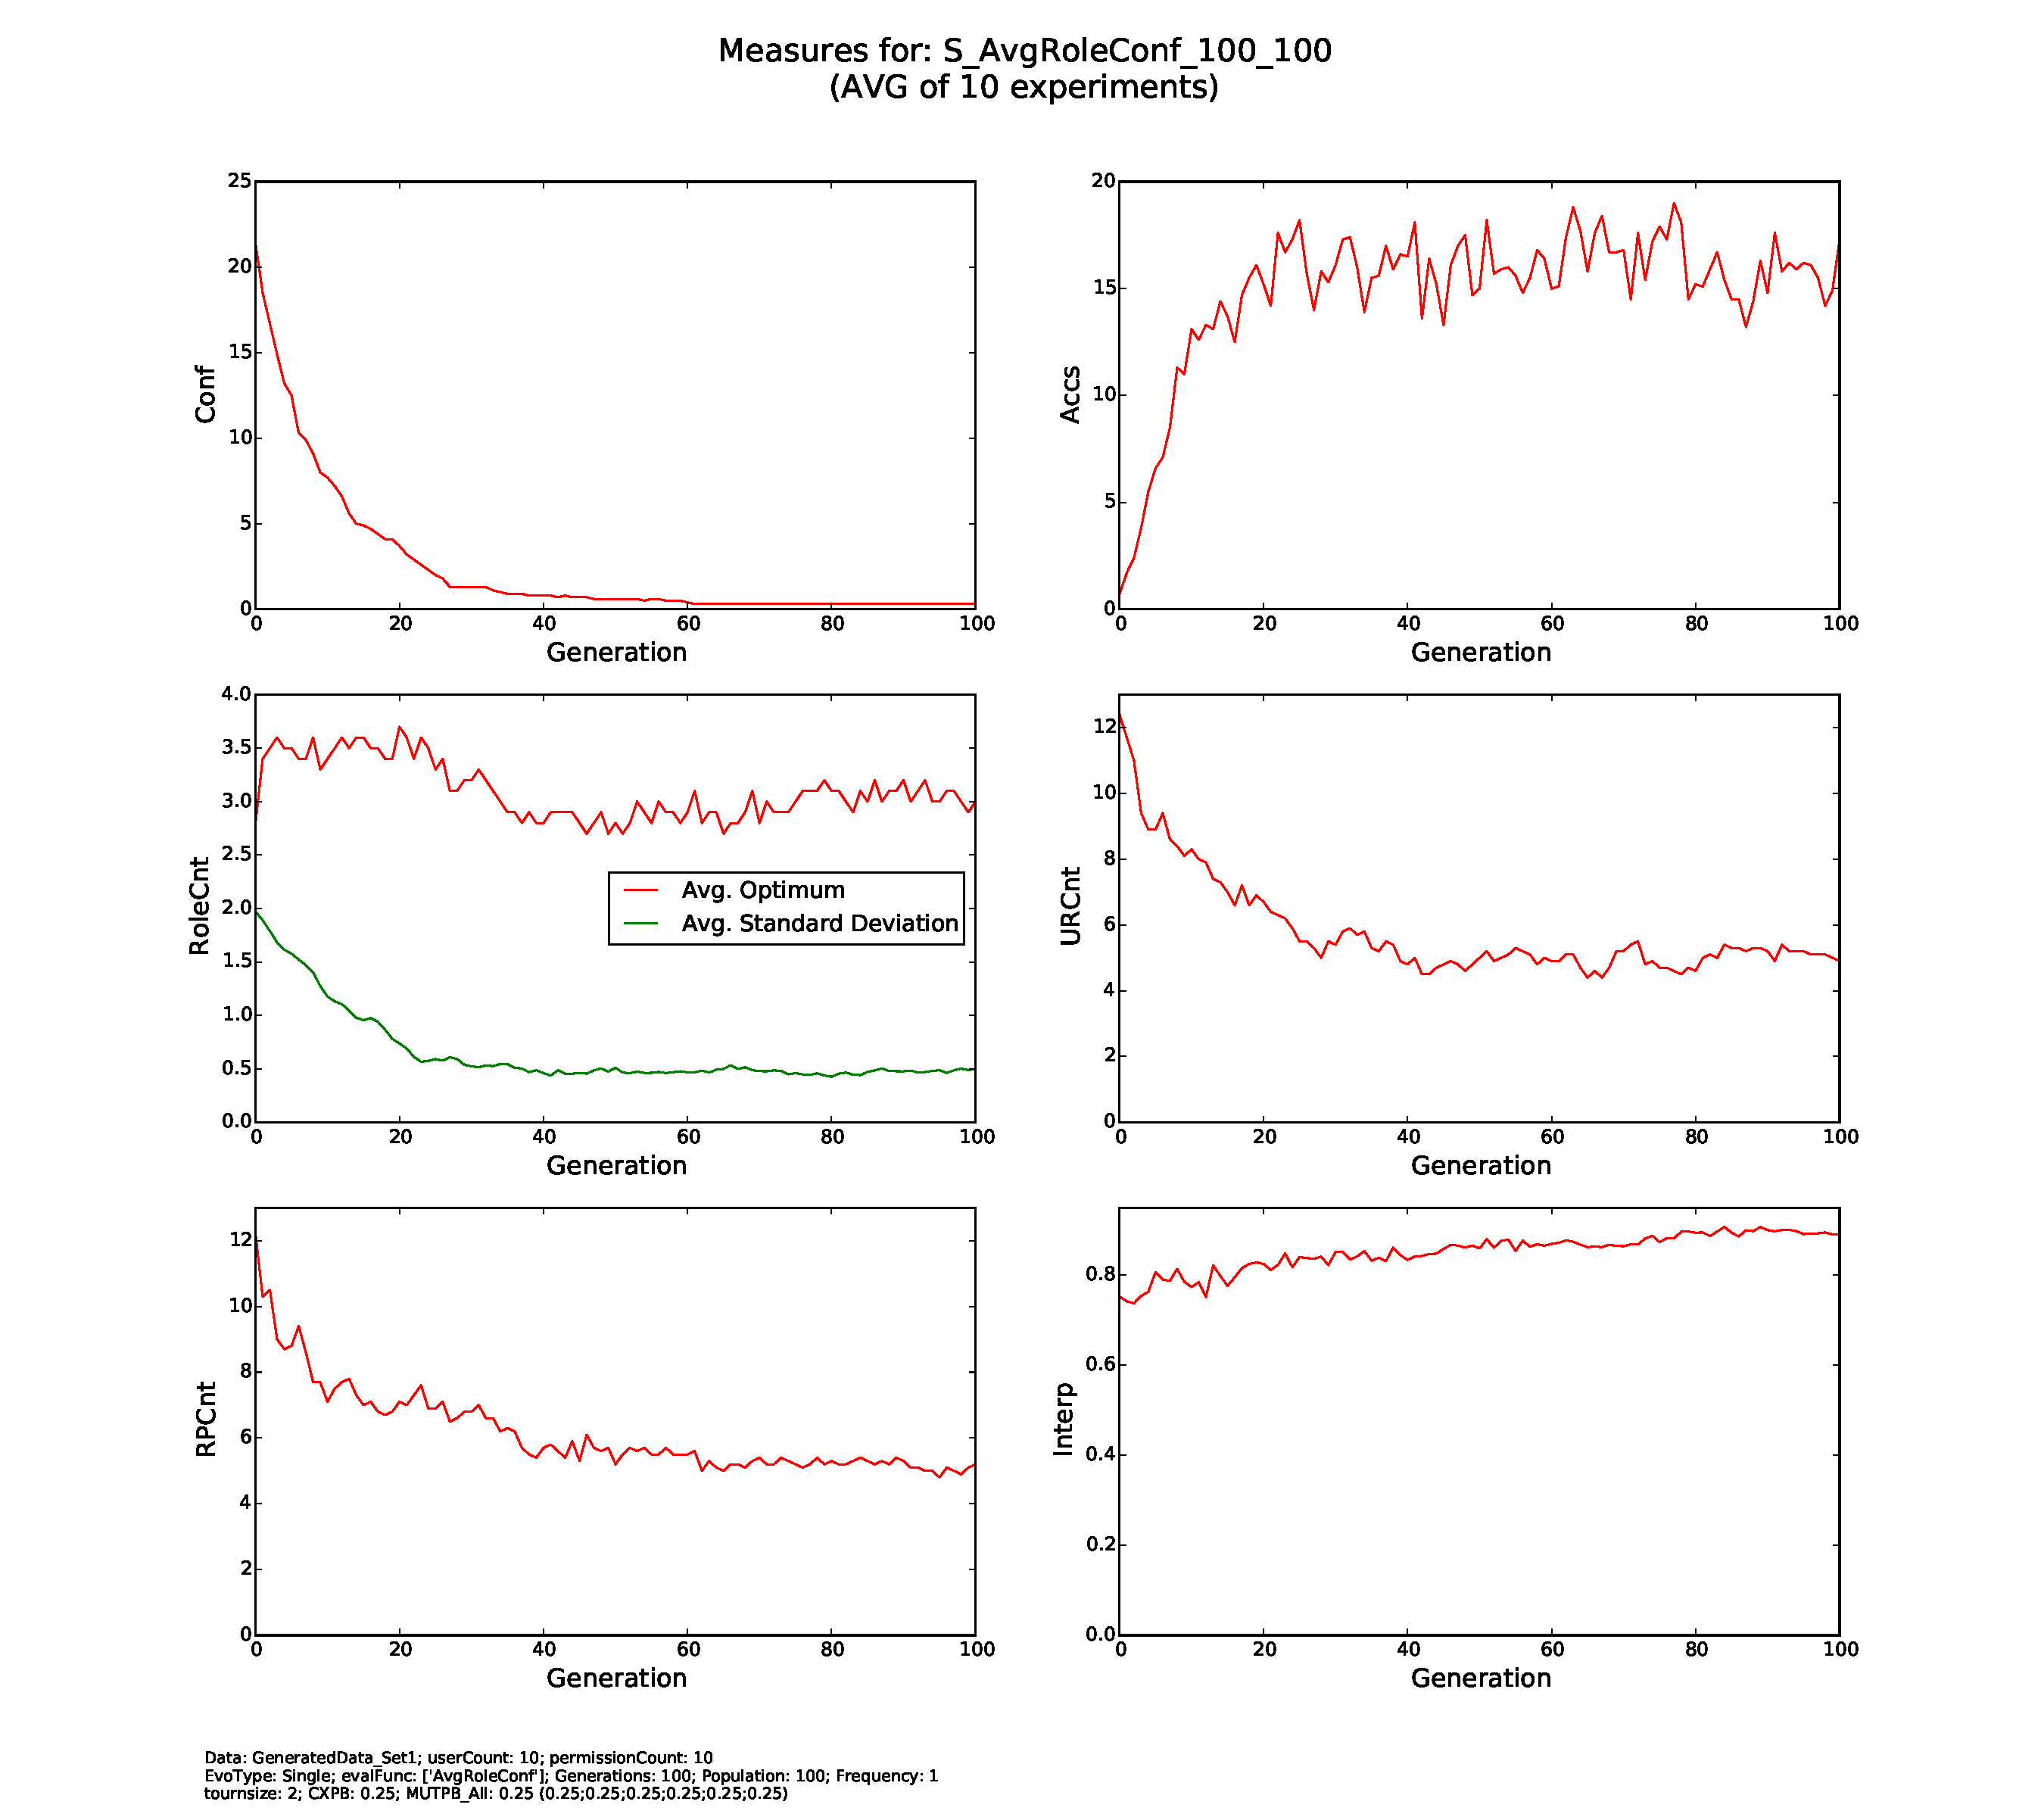
\includegraphics[scale=0.33, trim=4cm 2cm 4cm 0cm, clip=true]{exp1_avgConf}
		    \caption{EXPERIMENT 1c: Results of EvoRoleMiner with Fitness function $F=avg(G_{conf})$ on synthetic dataset 1 with setup in table \ref{tab:setup1}. From u.l. to l.r.: Confidentiality Violations, Availability Violations, Role Count, User-Role Assignments, Role-Permission Assignments, Interpretability.}
		    \label{fig:exp1_avgConf}
		\end{figure}
		
		\begin{figure}[H]
			\centering
		    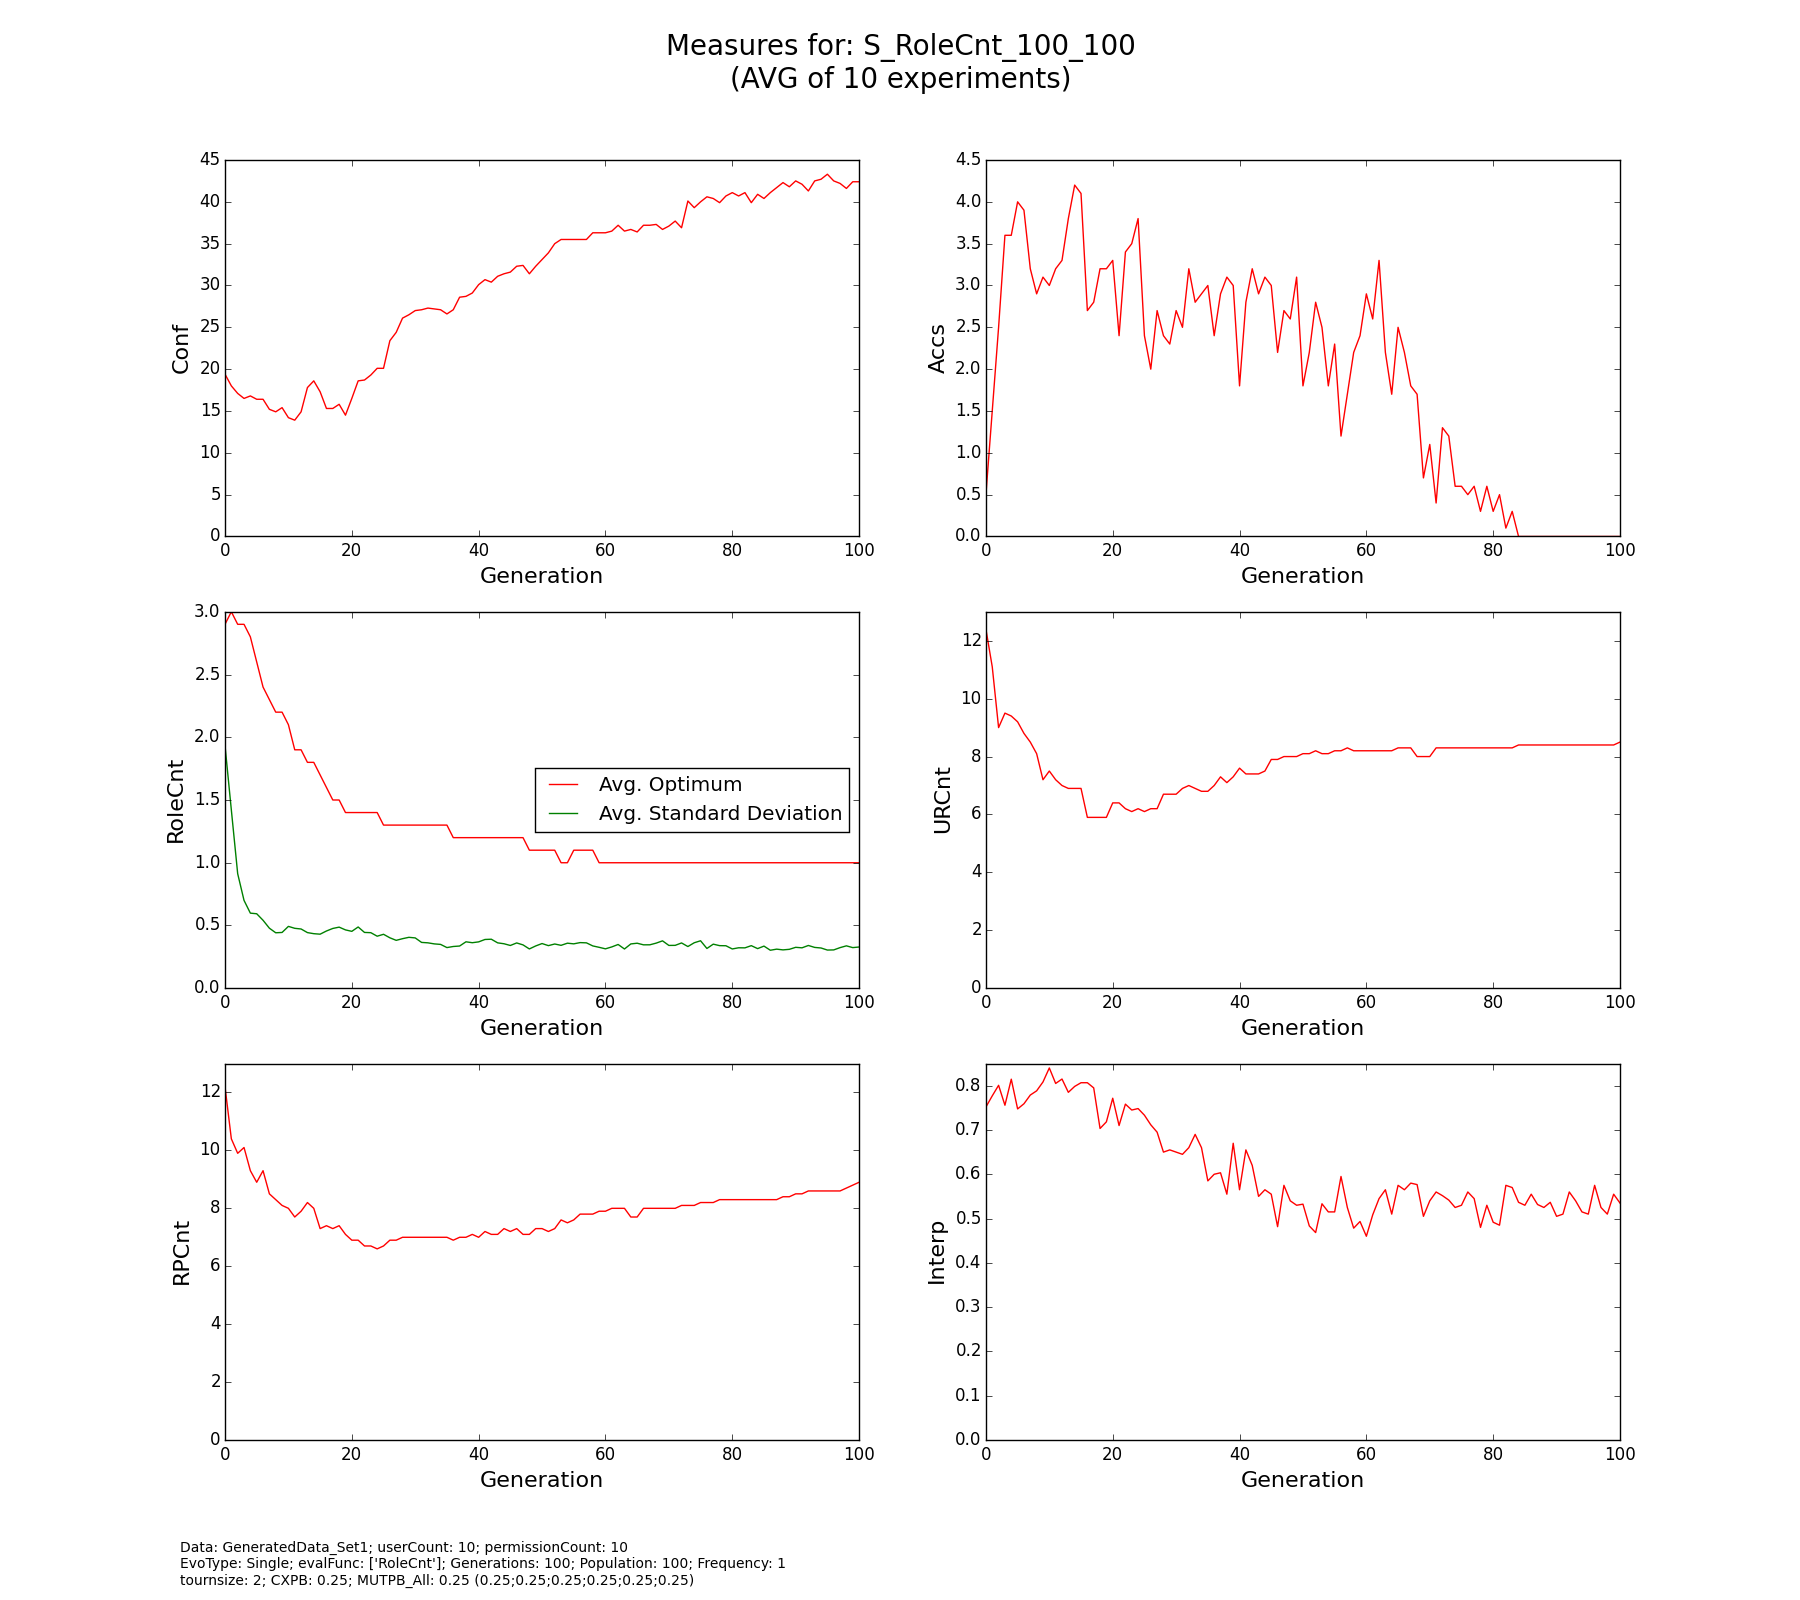
\includegraphics[scale=0.33, trim=4cm 2cm 4cm 0cm, clip=true]{exp1_roleCnt}
		    \caption{EXPERIMENT 1d: Results of EvoRoleMiner with Fitness function $F=|R|$ on synthetic dataset 1 with setup in table \ref{tab:setup1}. From u.l. to l.r.: Confidentiality Violations, Availability Violations, Role Count, User-Role Assignments, Role-Permission Assignments, Interpretability.}
		    \label{fig:exp1_roleCnt}
		\end{figure}
		
		\begin{figure}[H]
			\centering
		    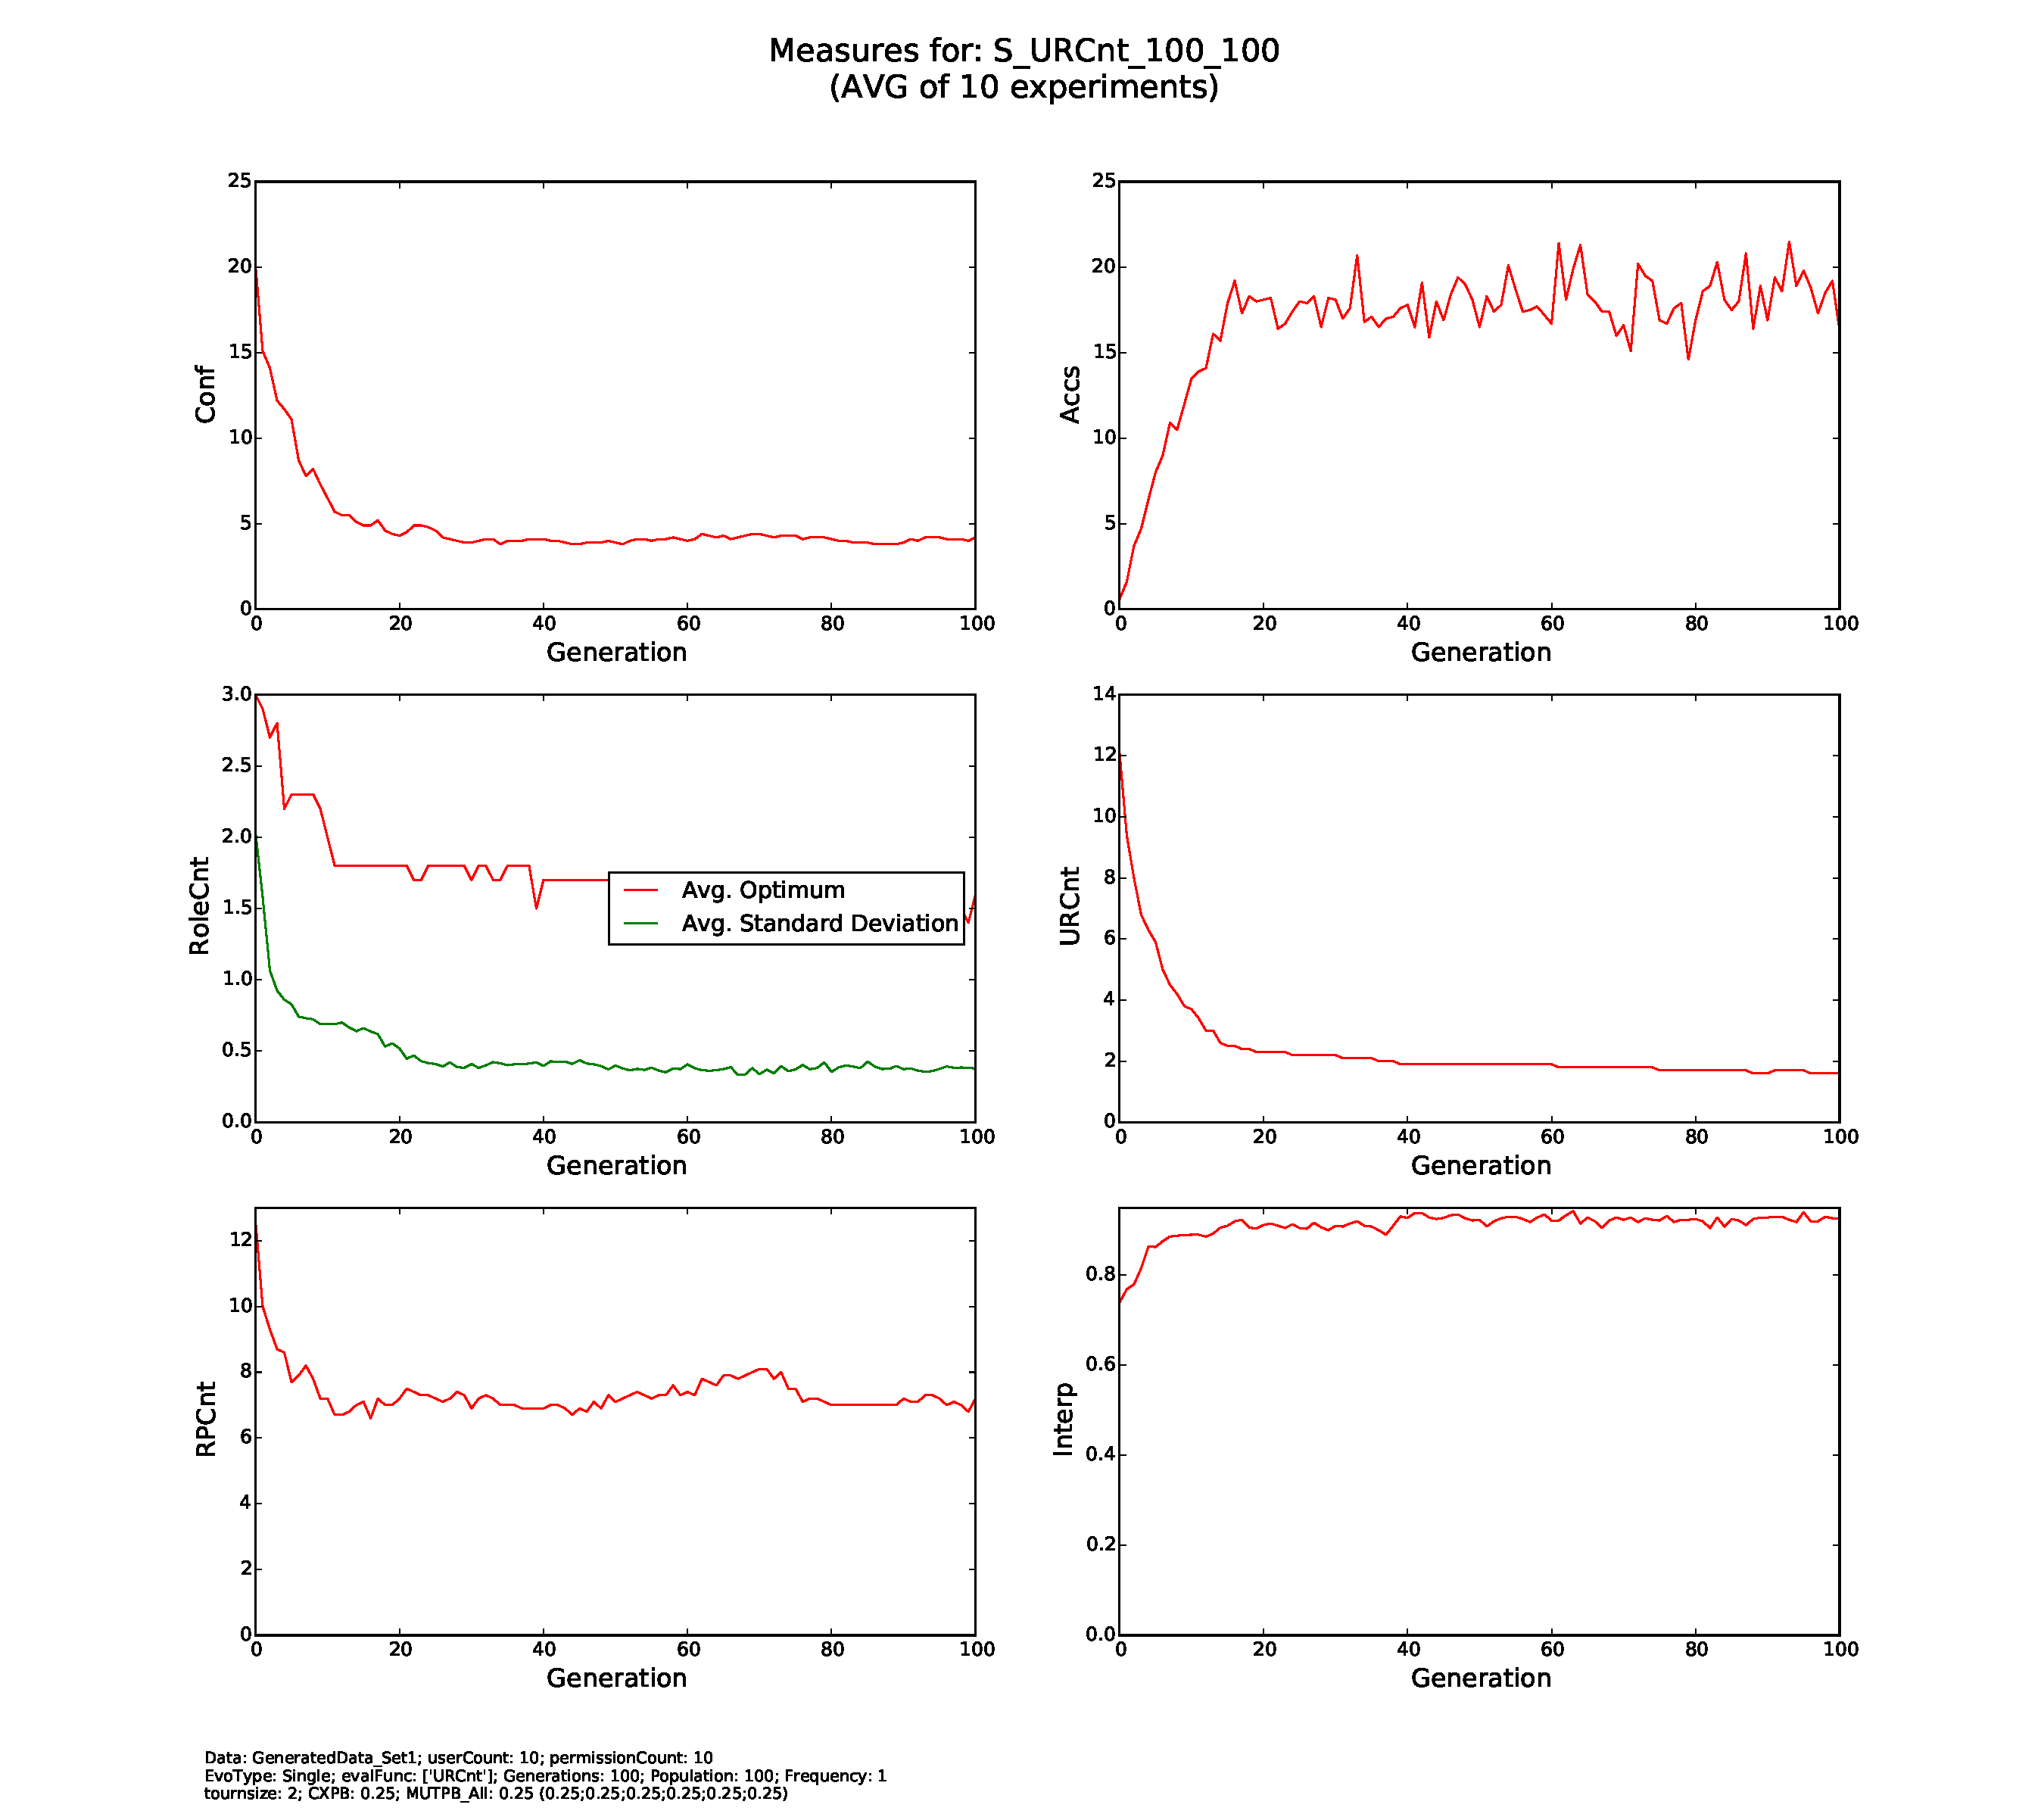
\includegraphics[scale=0.33, trim=4cm 2cm 4cm 0cm, clip=true]{exp1_urCnt}
		    \caption{EXPERIMENT 1e: Results of EvoRoleMiner with Fitness function $F=|UA|$ on synthetic dataset 1 with setup in table \ref{tab:setup1}. From u.l. to l.r.: Confidentiality Violations, Availability Violations, Role Count, User-Role Assignments, Role-Permission Assignments, Interpretability.}
		    \label{fig:exp1_urCnt}
		\end{figure}
		
		\begin{figure}[H]
		    \centering
		    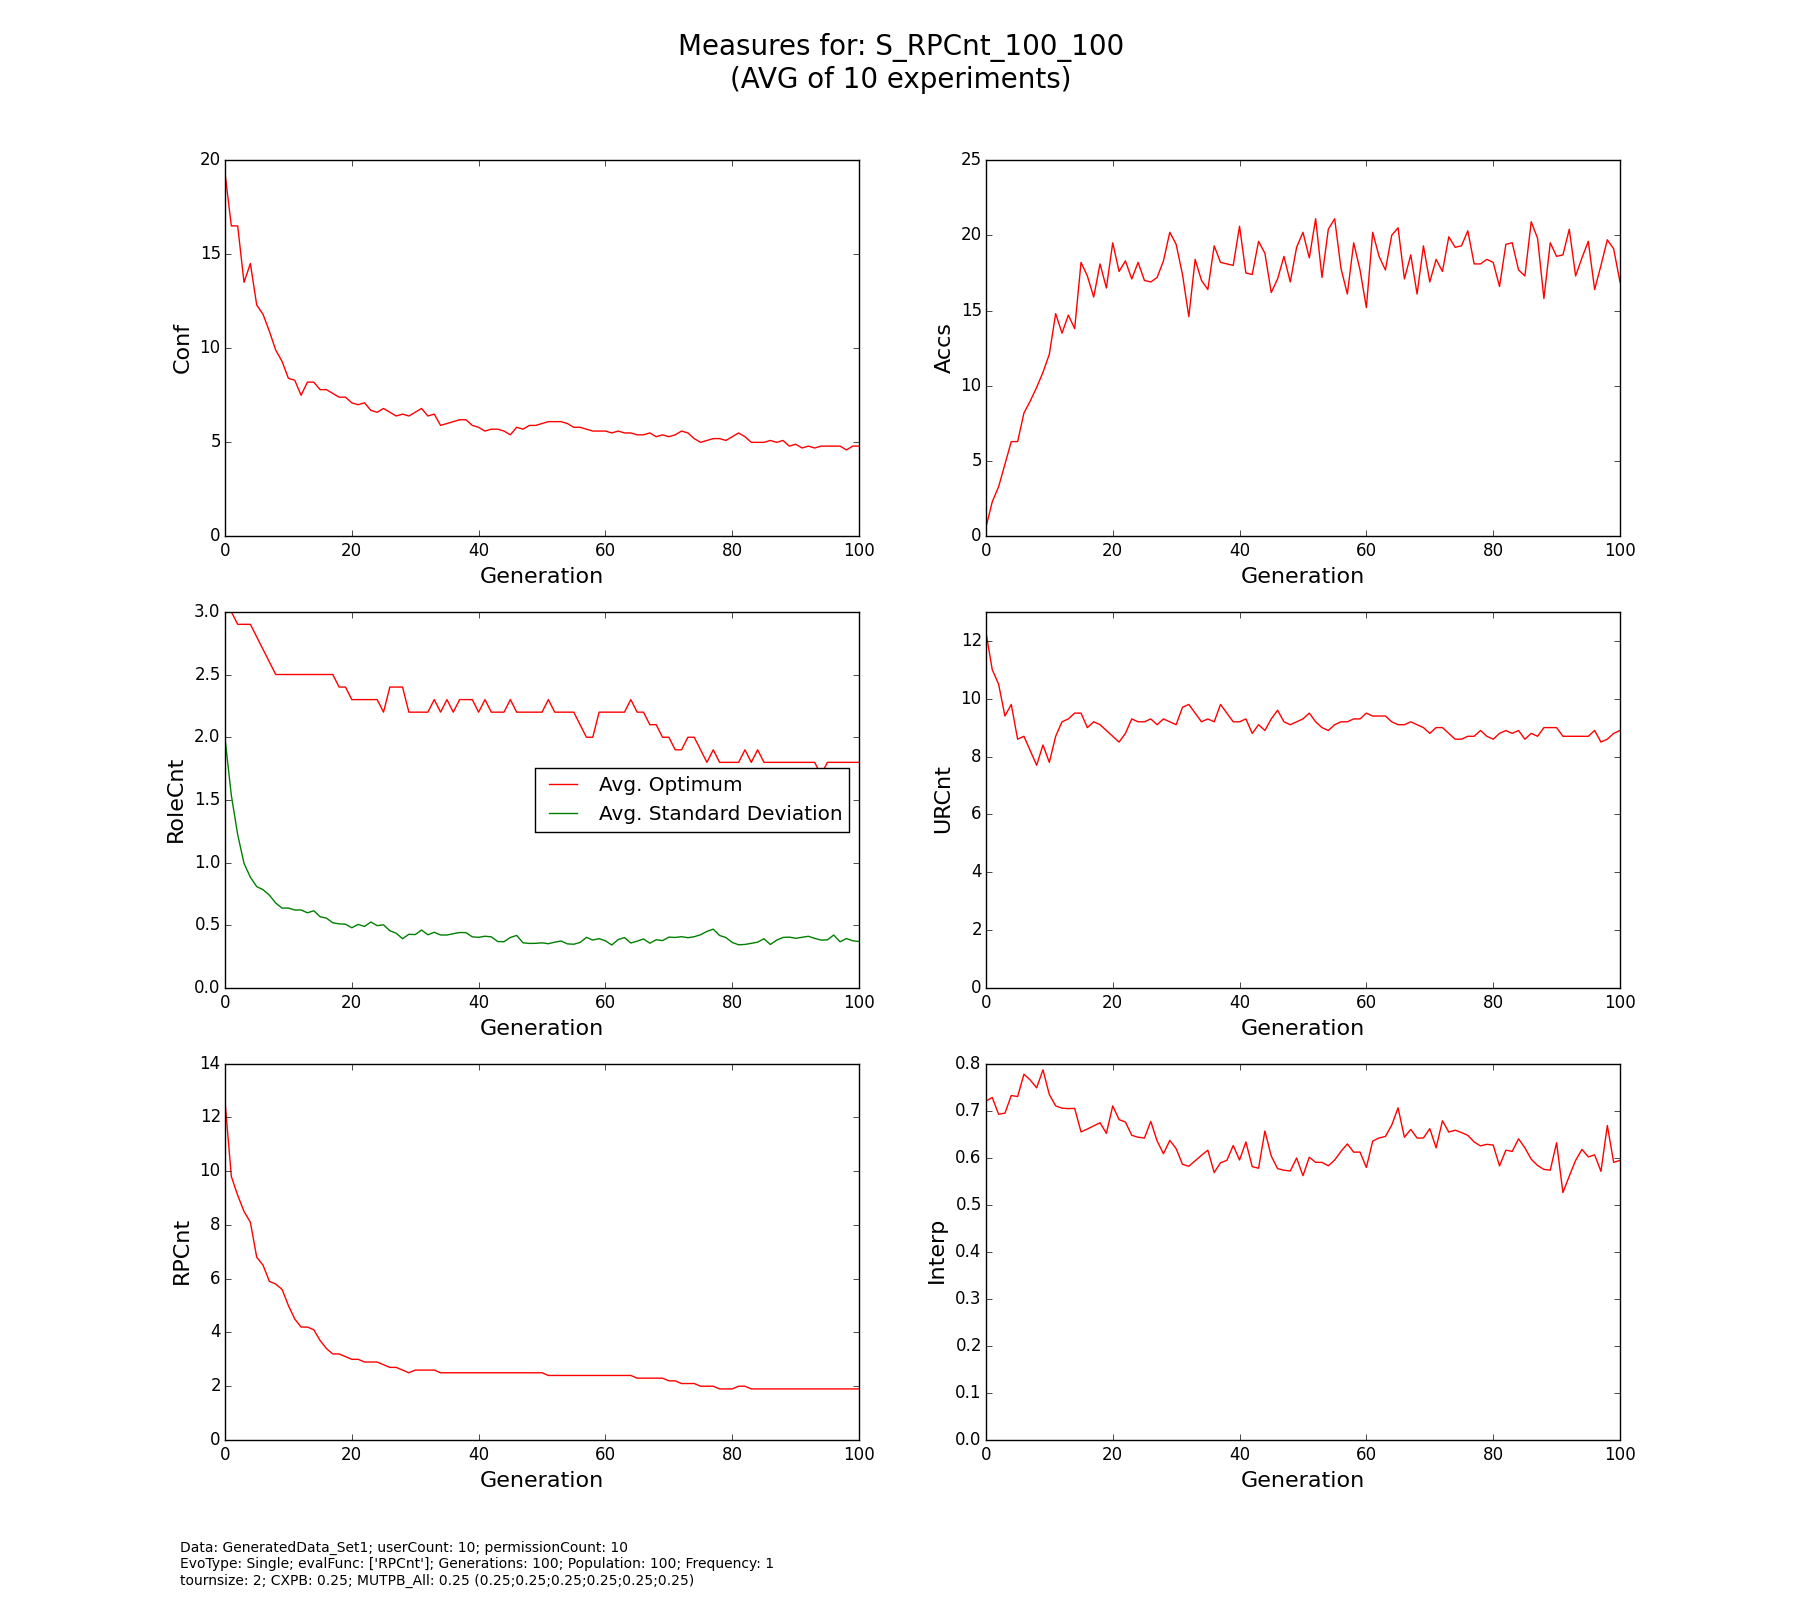
\includegraphics[scale=0.33, trim=4cm 2cm 4cm 0cm, clip=true]{exp1_rpCnt}
	    	\caption{EXPERIMENT 1f: Results of EvoRoleMiner with Fitness function $F=|PA|$ on synthetic dataset 1 with setup in table \ref{tab:setup1}. From u.l. to l.r.: Confidentiality Violations, Availability Violations, Role Count, User-Role Assignments, Role-Permission Assignments, Interpretability.}
	    	\label{fig:exp1_rpCnt}
	    \end{figure}
	
\section{Experiment 2a}
\label{sec:A_Exp2a}
	\subsection{Result Data}
	\label{sec:A_Exp2a_Data}	
		\begin{table}[H]
		\caption{Results of Experiment 2a: Synthetic Dataset 1, $F_{Basic}^{INT}$, Setup 1}
		\label{tab:A_Exp2a_Data}
			\begin{adjustbox}{max width=380pt,keepaspectratio,angle=90}
				\begin{tabular}{|l|l|l|l|l|l|l|l|l|l|l|}
					\rowcolor[HTML]{EFEFEF} 
					\hline
					Experiment & evals & Fitness\_Min & Fitness\_Max & Fitness\_Avg & Fitness\_Std & Conf\_Min & Conf\_Max & Conf\_Avg & Conf\_Std   & Accs\_Min \\ \hline
					1          & 424   & 0.377769019  & 1.149704375  & 0.426066102  & 0.112333904  & 4         & 40        & 5.842     & 4.785084743 & 0         \\ \hline
					2          & 443   & 0.377769019  & 1.221836815  & 0.433073354  & 0.120951333  & 3         & 42        & 6.068     & 5.067087526 & 0         \\ \hline
					3          & 449   & 0.377769019  & 1.204887663  & 0.436002483  & 0.129238799  & 3         & 44        & 6.226     & 5.437915409 & 0         \\ \hline
					4          & 423   & 0.377769019  & 0.962987781  & 0.428166732  & 0.110813532  & 2         & 34        & 5.836     & 4.625916558 & 0         \\ \hline
					5          & 404   & 0.377769019  & 1.18793851   & 0.432763618  & 0.123186393  & 2         & 40        & 6.109     & 5.244722967 & 0         \\ \hline
					6          & 458   & 0.377769019  & 1.141426882  & 0.428852621  & 0.115522095  & 3         & 40        & 5.926     & 4.787747278 & 0         \\ \hline
					7          & 434   & 0.377769019  & 1.135120221  & 0.427447024  & 0.109024379  & 3         & 41        & 5.758     & 4.503047413 & 0         \\ \hline
					8          & 482   & 0.377769019  & 1.194245171  & 0.428993023  & 0.121726637  & 3         & 45        & 5.962     & 5.30721735  & 0         \\ \hline
					9          & 423   & 0.377769019  & 1.152069373  & 0.422152266  & 0.107280322  & 3         & 42        & 5.686     & 4.499489304 & 0         \\ \hline
					10         & 435   & 0.377769019  & 1.117776902  & 0.428012929  & 0.114866488  & 2         & 35        & 5.898     & 4.766927312 & 0         \\ \hline\hline
					AVG        & 437.5 & 0.377769019  & 1.146799369  & 0.429153015  & 0.116494388  & 2.8       & 40.3      & 5.9311    & 4.902515586 & 0         \\ \hline
				\end{tabular}
			\end{adjustbox}
			\begin{adjustbox}{max width=380pt,keepaspectratio,angle=90}
				\begin{tabular}{|l|l|l|l|l|l|l|l|l|l|l|}
					\rowcolor[HTML]{EFEFEF} 
					\hline
					Experiment & Accs\_Max & Accs\_Avg & Accs\_Std   & RoleCnt\_Min & RoleCnt\_Max & RoleCnt\_Avg & RoleCnt\_Std & URCnt\_Min & URCnt\_Max & URCnt\_Avg \\ \hline
					1          & 10        & 3.214     & 1.101001362 & 2            & 4            & 2.121        & 0.363811765  & 9          & 24         & 9.6        \\ \hline
					2          & 11        & 3.256     & 1.185944349 & 2            & 4            & 2.143        & 0.382819801  & 9          & 22         & 9.656      \\ \hline
					3          & 12        & 3.241     & 1.189503678 & 2            & 4            & 2.149        & 0.410851555  & 9          & 23         & 9.741      \\ \hline
					4          & 12        & 3.313     & 1.296545796 & 2            & 4            & 2.12         & 0.345832329  & 9          & 18         & 9.599      \\ \hline
					5          & 10        & 3.23      & 1.170939794 & 2            & 4            & 2.139        & 0.379050129  & 9          & 21         & 9.665      \\ \hline
					6          & 12        & 3.221     & 1.11631492  & 2            & 4            & 2.133        & 0.388987146  & 9          & 21         & 9.663      \\ \hline
					7          & 13        & 3.326     & 1.341537923 & 2            & 4            & 2.123        & 0.365883861  & 9          & 24         & 9.61       \\ \hline
					8          & 14        & 3.218     & 1.153462613 & 2            & 4            & 2.129        & 0.366550133  & 8          & 21         & 9.655      \\ \hline
					9          & 13        & 3.211     & 1.086498504 & 2            & 4            & 2.109        & 0.348021551  & 9          & 22         & 9.544      \\ \hline
					10         & 13        & 3.201     & 1.163872416 & 2            & 4            & 2.134        & 0.382157036  & 9          & 20         & 9.649      \\ \hline\hline
					AVG        & 12        & 3.2431    & 1.180562135 & 2            & 4            & 2.13         & 0.373396531  & 8.9        & 21.6       & 9.6382     \\ \hline
				\end{tabular}	
			\end{adjustbox}
			\begin{adjustbox}{max width=380pt,keepaspectratio,angle=90}
				\begin{tabular}{|l|l|l|l|l|l|l|l|l|l|l|}
					\rowcolor[HTML]{EFEFEF} 
					\hline
					Experiment & URCnt\_Std  & RPCnt\_Min & RPCnt\_Max & RPCnt\_Avg & RPCnt\_Std  & Interp\_Min & Interp\_Max & Interp\_Avg & Interp\_Std & Runtime     \\ \hline
					1          & 1.722788437 & 8          & 22         & 9.571      & 1.872153573 & 0.45        & 1           & 0.953491667 & 0.123598094 & 406.153624  \\ \hline
					2          & 1.695188485 & 8          & 21         & 9.66       & 1.901157542 & 0.333333333 & 1           & 0.9512      & 0.123606472 & 413.456295  \\ \hline
					3          & 1.976339799 & 8          & 23         & 9.68       & 2.021781393 & 0.3         & 1           & 0.951525    & 0.124034468 & 386.242228  \\ \hline
					4          & 1.582466113 & 8          & 21         & 9.511      & 1.701728239 & 0.25        & 1           & 0.951675    & 0.127128161 & 0           \\ \hline
					5          & 1.791863555 & 8          & 22         & 9.624      & 1.833745893 & 0           & 1           & 0.951616667 & 0.127101874 & 254.715648  \\ \hline
					6          & 1.799841938 & 8          & 23         & 9.576      & 1.824342073 & 0.333333333 & 1           & 0.95085     & 0.126742739 & 309.848566  \\ \hline
					7          & 1.716362433 & 8          & 21         & 9.518      & 1.77191309  & 0.25        & 1           & 0.955308333 & 0.118857767 & 303.092263  \\ \hline
					8          & 1.827559849 & 8          & 23         & 9.565      & 1.809910219 & 0.3         & 1           & 0.951008333 & 0.130667187 & 315.908143  \\ \hline
					9          & 1.674533965 & 8          & 22         & 9.481      & 1.648526312 & 0.25        & 1           & 0.958041667 & 0.122806243 & 325.160113  \\ \hline
					10         & 1.748656341 & 7          & 23         & 9.583      & 1.830057649 & 0.333333333 & 1           & 0.949616667 & 0.12924242  & 312.639989  \\ \hline\hline
					AVG        & 1.753560091 & 7.9        & 22.1       & 9.5769     & 1.821531598 & 0.28        & 1           & 0.952433333 & 0.125378543 & 336.3574299 \\ \hline						
				\end{tabular}
			\end{adjustbox}	
		\end{table}
	\subsection{Result Visualizations}
	\label{sec:A_Exp2a_Diagrams}
		\begin{figure}[H]
			\centering
			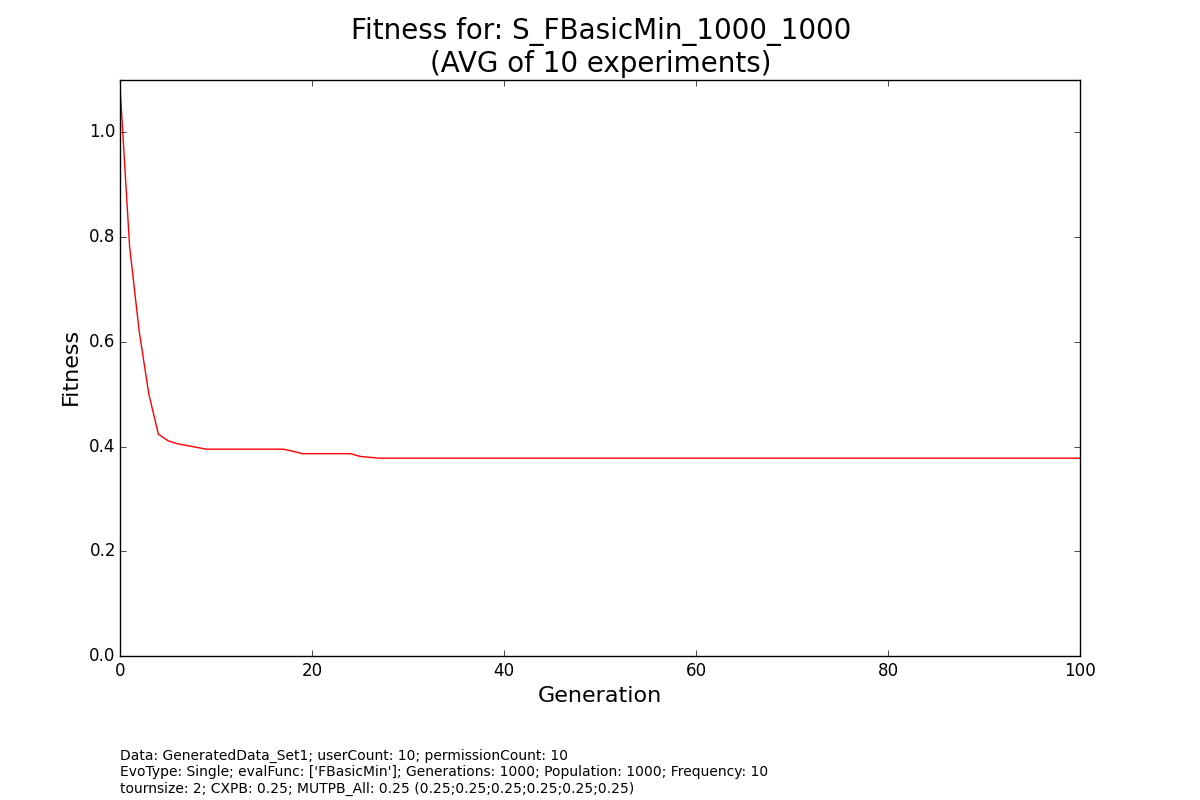
\includegraphics[scale=0.4, trim=0cm 2cm 0cm 0cm, clip=true]{exp2a_Fitness}
			\caption{EXPERIMENT 2a: Average minimum Fitness Graph of ten experiments with fitness function $F_{basic}^{min}$ and synthetic dataset 1}
			\label{fig:exp2afitness}
		\end{figure}
	
\section{Experiment 2b}
\label{sec:A_Exp2b}
	\subsection{Result Data}
	\label{sec:A_Exp2b_Data}
		\begin{table}[H]
			\caption{Results of Experiment 2a: Synthetic Dataset 1, $F_{Edge}^{INT}$, Setup 1}
			\label{tab:A_Exp2b_Data}
			\begin{adjustbox}{max width=380pt,keepaspectratio,angle=90}
				\begin{tabular}{|l|l|l|l|l|l|l|l|l|l|l|}
					\rowcolor[HTML]{EFEFEF} 
					\hline
					Experiment & evals & Fitness\_Min & Fitness\_Max & Fitness\_Avg & Fitness\_Std & Conf\_Min & Conf\_Max & Conf\_Avg & Conf\_Std   & Accs\_Min \\ \hline
					1          & 448   & 0.151957621  & 0.950218091  & 0.197838357  & 0.112719345  & 3         & 40        & 5.653     & 4.484929319 & 0         \\ \hline
					2          & 468   & 0.151957621  & 0.910013124  & 0.196031551  & 0.106774032  & 3         & 39        & 5.597     & 4.268558422 & 0         \\ \hline
					3          & 414   & 0.151957621  & 0.954900441  & 0.193278273  & 0.108811647  & 3         & 41        & 5.53      & 4.379394935 & 0         \\ \hline
					4          & 446   & 0.151957621  & 0.904052983  & 0.195771496  & 0.106907863  & 4         & 38        & 5.561     & 4.295844387 & 0         \\ \hline
					5          & 418   & 0.151957621  & 0.828515985  & 0.193427922  & 0.109222984  & 2         & 34        & 5.479     & 4.28830491  & 0         \\ \hline
					6          & 430   & 0.151957621  & 0.931835212  & 0.198015858  & 0.114541813  & 4         & 39        & 5.692     & 4.632832395 & 0         \\ \hline
					7          & 444   & 0.151957621  & 0.859165667  & 0.193724664  & 0.107789762  & 3         & 36        & 5.495     & 4.325734042 & 0         \\ \hline
					8          & 450   & 0.151957621  & 0.957217792  & 0.192751294  & 0.102121551  & 2         & 35        & 5.418     & 3.887322472 & 0         \\ \hline
					9          & 434   & 0.151957621  & 0.893063972  & 0.196081224  & 0.10881912   & 4         & 38        & 5.564     & 4.240271689 & 0         \\ \hline
					10         & 434   & 0.139106065  & 0.863263264  & 0.177983839  & 0.10480901   & 0         & 33        & 1.44      & 4.305159695 & 0         \\ \hline\hline
					AVG        & 438.6 & 0.150672465  & 0.905224653  & 0.193490448  & 0.108251713  & 2.8       & 37.3      & 5.1429    & 4.310835227 & 0         \\ \hline
				\end{tabular}
			\end{adjustbox}
			\begin{adjustbox}{max width=380pt,keepaspectratio,angle=90}
				\begin{tabular}{|l|l|l|l|l|l|l|l|l|l|l|}
					\rowcolor[HTML]{EFEFEF} 
					\hline
					Experiment & Accs\_Max & Accs\_Avg & Accs\_Std   & RoleCnt\_Min & RoleCnt\_Max & RoleCnt\_Avg & RoleCnt\_Std & URCnt\_Min & URCnt\_Max & URCnt\_Avg \\ \hline
					1          & 8         & 0.246     & 0.971331046 & 3            & 5            & 3.123        & 0.334471224  & 9          & 22         & 10.583     \\ \hline
					2          & 9         & 0.28      & 1.051475154 & 3            & 4            & 3.098        & 0.297314648  & 10         & 19         & 10.531     \\ \hline
					3          & 10        & 0.218     & 0.976972876 & 3            & 4            & 3.094        & 0.291828717  & 10         & 19         & 10.508     \\ \hline
					4          & 8         & 0.296     & 1.090130267 & 3            & 4            & 3.102        & 0.302648311  & 9          & 20         & 10.488     \\ \hline
					5          & 9         & 0.272     & 1.046907828 & 3            & 5            & 3.095        & 0.296605799  & 9          & 19         & 10.506     \\ \hline
					6          & 9         & 0.246     & 0.956809281 & 3            & 5            & 3.111        & 0.317299543  & 10         & 19         & 10.545     \\ \hline
					7          & 9         & 0.292     & 1.090291704 & 3            & 4            & 3.09         & 0.28618176   & 9          & 19         & 10.513     \\ \hline
					8          & 9         & 0.242     & 0.953643539 & 3            & 4            & 3.113        & 0.316592798  & 10         & 18         & 10.538     \\ \hline
					9          & 10        & 0.275     & 1.111474246 & 3            & 5            & 3.111        & 0.320435641  & 10         & 23         & 10.57      \\ \hline
					10         & 10        & 0.231     & 0.838831926 & 4            & 5            & 4.087        & 0.281835058  & 10         & 19         & 10.492     \\ \hline\hline
					AVG        & 9.1       & 0.2598    & 1.008786787 & 3.1          & 4.5          & 3.2024       & 0.30452135   & 9.6        & 19.7       & 10.5274    \\ \hline
				\end{tabular}	
			\end{adjustbox}
			\begin{adjustbox}{max width=380pt,keepaspectratio,angle=90}
				\begin{tabular}{|l|l|l|l|l|l|l|l|l|l|l|}
					\rowcolor[HTML]{EFEFEF} 
					\hline
					Experiment & URCnt\_Std  & RPCnt\_Min & RPCnt\_Max & RPCnt\_Avg & RPCnt\_Std  & Interp\_Min & Interp\_Max & Interp\_Avg & Interp\_Std & Runtime\_Sum \\ \hline
					1          & 1.574519292 & 11         & 21         & 12.522     & 1.583513814 & 0.5         & 1           & 0.967731667 & 0.087395377 & 347.57399    \\ \hline
					2          & 1.484263791 & 11         & 21         & 12.424     & 1.465682094 & 0.5         & 1           & 0.965483333 & 0.090418716 & 380.48422    \\ \hline
					3          & 1.477137773 & 11         & 21         & 12.431     & 1.45644739  & 0.25        & 1           & 0.969391667 & 0.084816006 & 355.304555   \\ \hline
					4          & 1.404227902 & 10         & 21         & 12.465     & 1.555241139 & 0.5         & 1           & 0.968441667 & 0.085626624 & 328.616984   \\ \hline
					5          & 1.499988    & 10         & 20         & 12.411     & 1.467678098 & 0.5         & 1           & 0.970053333 & 0.085864961 & 336.439346   \\ \hline
					6          & 1.477827798 & 11         & 22         & 12.516     & 1.680994943 & 0.45        & 1           & 0.969331667 & 0.084649838 & 321.674719   \\ \hline
					7          & 1.527688123 & 11         & 21         & 12.364     & 1.359229193 & 0.333333333 & 1           & 0.968058333 & 0.090619439 & 318.312672   \\ \hline
					8          & 1.45827158  & 11         & 24         & 12.475     & 1.556076798 & 0.45        & 1           & 0.971433333 & 0.079903073 & 326.259763   \\ \hline
					9          & 1.644718821 & 11         & 20         & 12.451     & 1.457257355 & 0.36        & 1           & 0.964068333 & 0.096519867 & 331.524604   \\ \hline
					10         & 1.398547818 & 14         & 25         & 17.336     & 1.323292863 & 0.6         & 1           & 0.974785    & 0.068962517 & 387.358279   \\ \hline\hline
					AVG        & 1.49471909  & 11.1       & 21.6       & 12.9395    & 1.490541369 & 0.444333333 & 1           & 0.968877833 & 0.085477642 & 343.3549132  \\ \hline
				\end{tabular}
			\end{adjustbox}	
		\end{table}
	\subsection{Result Visualizations}
	\label{sec:A_Exp2b_Diagrams}
		\begin{figure}[H]
			\centering
			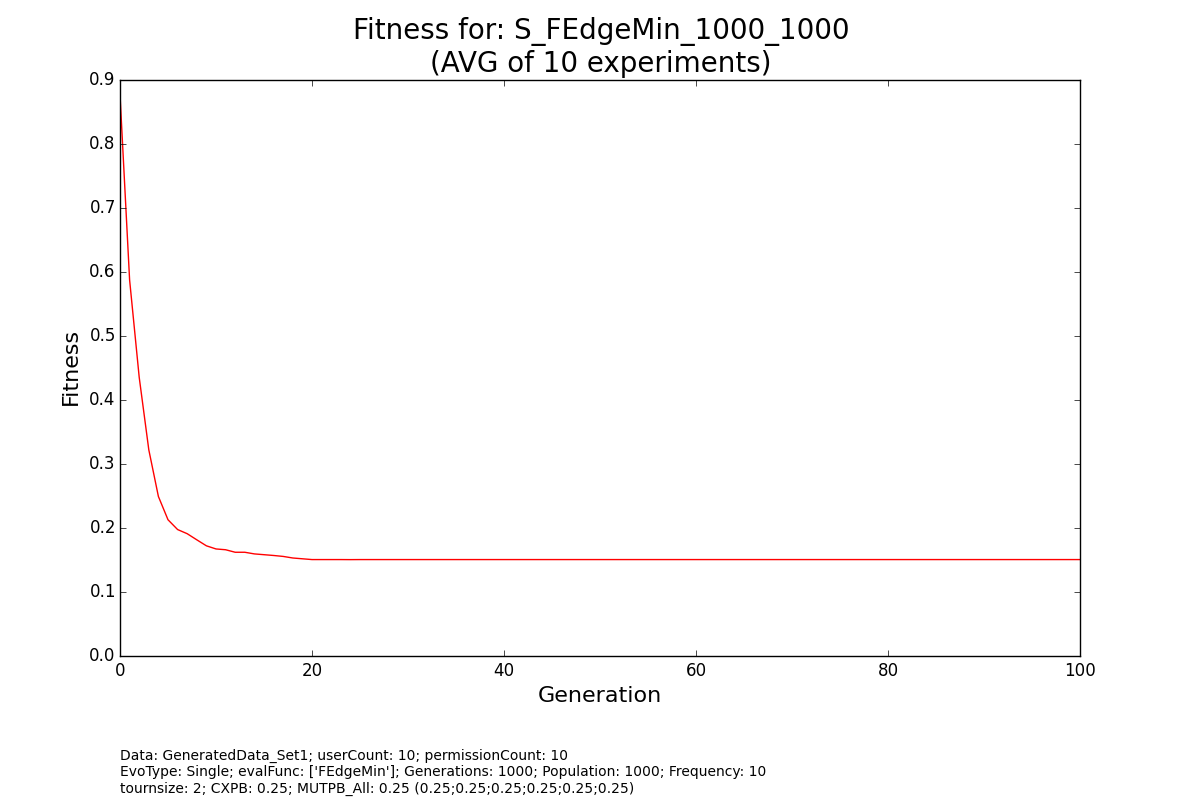
\includegraphics[scale=0.4, trim=0cm 2cm 0cm 0cm, clip=true]{exp2b_Fitness}
			\caption{EXPERIMENT 2b: Average minimum Fitness Graph of ten experiments with fitness function $F_{edge}^{min}$ and synthetic dataset 1}
			\label{fig:exp2bfitness}
		\end{figure}
		
\section{Experiment 2c}
\label{sec:A_Exp2c}
	\subsection{Result Data}
	\label{sec:A_Exp2c_Data}
		\begin{table}[H]
			\caption{Results of Experiment 2c: Healthcare Dataset, $F_{Basic}^{INT}$, Setup 1}
			\label{tab:A_Exp2c_Data}
			\begin{adjustbox}{max width=380pt,keepaspectratio,angle=90}
				\begin{tabular}{|l|l|l|l|l|l|l|l|l|l|l|}
					\rowcolor[HTML]{EFEFEF} 
					\hline
					Experiment & evals & Fitness\_Min & Fitness\_Max & Fitness\_Avg & Fitness\_Std & Conf\_Min & Conf\_Max & Conf\_Avg & Conf\_Std   & Accs\_Min \\ \hline
					1          & 438   & 0.130323897  & 0.615999032  & 0.151347383  & 0.062477382  & 0         & 301       & 16.692    & 37.71603288 & 63        \\ \hline
					2          & 458   & 0.130323897  & 0.73341388   & 0.157447219  & 0.077672584  & 5         & 384       & 20.391    & 47.67792067 & 53        \\ \hline
					3          & 430   & 0.130323897  & 0.674437884  & 0.15165764   & 0.061900488  & 0         & 354       & 16.864    & 37.7087192  & 36        \\ \hline
					4          & 432   & 0.130323897  & 0.67147639   & 0.15386933   & 0.066658348  & 0         & 365       & 18.377    & 40.80447121 & 36        \\ \hline
					5          & 419   & 0.130323897  & 0.635496057  & 0.154462113  & 0.068817039  & 5         & 315       & 18.572    & 41.44727755 & 52        \\ \hline
					6          & 429   & 0.130323897  & 0.606344306  & 0.155570018  & 0.071631728  & 1         & 300       & 19.096    & 43.8827846  & 58        \\ \hline
					7          & 394   & 0.130323897  & 0.679098455  & 0.151950346  & 0.067782347  & 0         & 351       & 17.278    & 41.49003153 & 41        \\ \hline
					8          & 446   & 0.130323897  & 0.705846916  & 0.15379811   & 0.068870807  & 5         & 370       & 18.383    & 42.26594742 & 45        \\ \hline
					9          & 429   & 0.154335484  & 0.695665704  & 0.177067085  & 0.066169436  & 15        & 364       & 33.61     & 39.63107241 & 44        \\ \hline
					10         & 427   & 0.130323897  & 0.642329969  & 0.154207422  & 0.06740591   & 5         & 336       & 18.355    & 41.13041423 & 56        \\ \hline\hline
					AVG        & 430.2 & 0.132725056  & 0.666010859  & 0.156137667  & 0.067938607  & 3.6       & 344       & 19.7618   & 41.37546717 & 48.4      \\ \hline
				\end{tabular}
			\end{adjustbox}
			\begin{adjustbox}{max width=380pt,keepaspectratio,angle=90}
				\begin{tabular}{|l|l|l|l|l|l|l|l|l|l|l|}
					\rowcolor[HTML]{EFEFEF} 
					\hline
					Experiment & Accs\_Max & Accs\_Avg & Accs\_Std   & RoleCnt\_Min & RoleCnt\_Max & RoleCnt\_Avg & RoleCnt\_Std & URCnt\_Min & URCnt\_Max & URCnt\_Avg \\ \hline
					1          & 166       & 113.959   & 9.677981143 & 2            & 4            & 2.116        & 0.358530333  & 45         & 104        & 55.021     \\ \hline
					2          & 166       & 113.472   & 10.66954619 & 2            & 5            & 2.142        & 0.392219326  & 61         & 126        & 65.536     \\ \hline
					3          & 166       & 114.112   & 10.06804132 & 2            & 4            & 2.113        & 0.352464183  & 54         & 110        & 61.993     \\ \hline
					4          & 166       & 113.609   & 10.3082549  & 2            & 4            & 2.12         & 0.36         & 60         & 111        & 64.862     \\ \hline
					5          & 166       & 113.74    & 10.23964843 & 2            & 4            & 2.129        & 0.392885479  & 60         & 122        & 65.298     \\ \hline
					6          & 194       & 113.894   & 11.18028461 & 2            & 4            & 2.137        & 0.382401621  & 51         & 115        & 57.558     \\ \hline
					7          & 142       & 113.41    & 9.154993173 & 2            & 4            & 2.118        & 0.352244233  & 50         & 101        & 58.511     \\ \hline
					8          & 166       & 113.295   & 9.809280045 & 2            & 4            & 2.126        & 0.363488652  & 61         & 121        & 65.013     \\ \hline
					9          & 164       & 112.174   & 9.37879118  & 2            & 4            & 2.121        & 0.361052628  & 44         & 104        & 50.491     \\ \hline
					10         & 163       & 113.808   & 9.832148087 & 2            & 4            & 2.131        & 0.37126675   & 62         & 119        & 65.25      \\ \hline\hline
					AVG        & 165.9     & 113.5473  & 10.03189691 & 2            & 4.1          & 2.1253       & 0.368655321  & 54.8       & 113.3      & 60.9533    \\ \hline
				\end{tabular}	
			\end{adjustbox}
			\begin{adjustbox}{max width=380pt,keepaspectratio,angle=90}
				\begin{tabular}{|l|l|l|l|l|l|l|l|l|l|l|}
					\rowcolor[HTML]{EFEFEF} 
					\hline
					Experiment & URCnt\_Std  & RPCnt\_Min & RPCnt\_Max & RPCnt\_Avg & RPCnt\_Std  & Interp\_Min & Interp\_Max & Interp\_Avg & Interp\_Std & Runtime     \\ \hline
					1          & 7.009319439 & 65         & 120        & 67.974     & 6.876577928 & 0           & 0           & 0           & 0           & 673.170894  \\ \hline
					2          & 7.75646208  & 48         & 105        & 58.294     & 8.528866513 & 0           & 0           & 0           & 0           & 738.401978  \\ \hline
					3          & 6.618833054 & 65         & 118        & 67.965     & 6.670215514 & 0           & 0           & 0           & 0           & 651.093222  \\ \hline
					4          & 6.791830092 & 64         & 122        & 67.961     & 7.148389959 & 0           & 0           & 0           & 0           & 671.645715  \\ \hline
					5          & 7.580844016 & 54         & 118        & 62.096     & 8.028498241 & 0           & 0           & 0           & 0           & 646.72621   \\ \hline
					6          & 7.605040171 & 64         & 121        & 68.416     & 7.439014989 & 0           & 0           & 0           & 0           & 659.20267   \\ \hline
					7          & 7.017825803 & 65         & 120        & 68.074     & 6.856422099 & 0           & 0           & 0           & 0           & 635.65854   \\ \hline
					8          & 7.236078427 & 63         & 125        & 67.672     & 6.86239142  & 0           & 0           & 0           & 0           & 651.406479  \\ \hline
					9          & 7.509721633 & 66         & 121        & 69.12      & 6.836929135 & 0           & 0           & 0           & 0           & 661.926049  \\ \hline
					10         & 7.231839323 & 54         & 115        & 64.092     & 7.749679735 & 0           & 0           & 0           & 0           & 651.49447   \\ \hline\hline
					AVG        & 7.235779404 & 60.8       & 118.5      & 66.1664    & 7.299698553 & 0           & 0           & 0           & 0           & 664.0726227 \\ \hline
				\end{tabular}
			\end{adjustbox}	
		\end{table}
	\subsection{Result Visualizations}
	\label{sec:A_Exp2c_Diagrams}
		\begin{figure}[H]
	    	\centering
	    	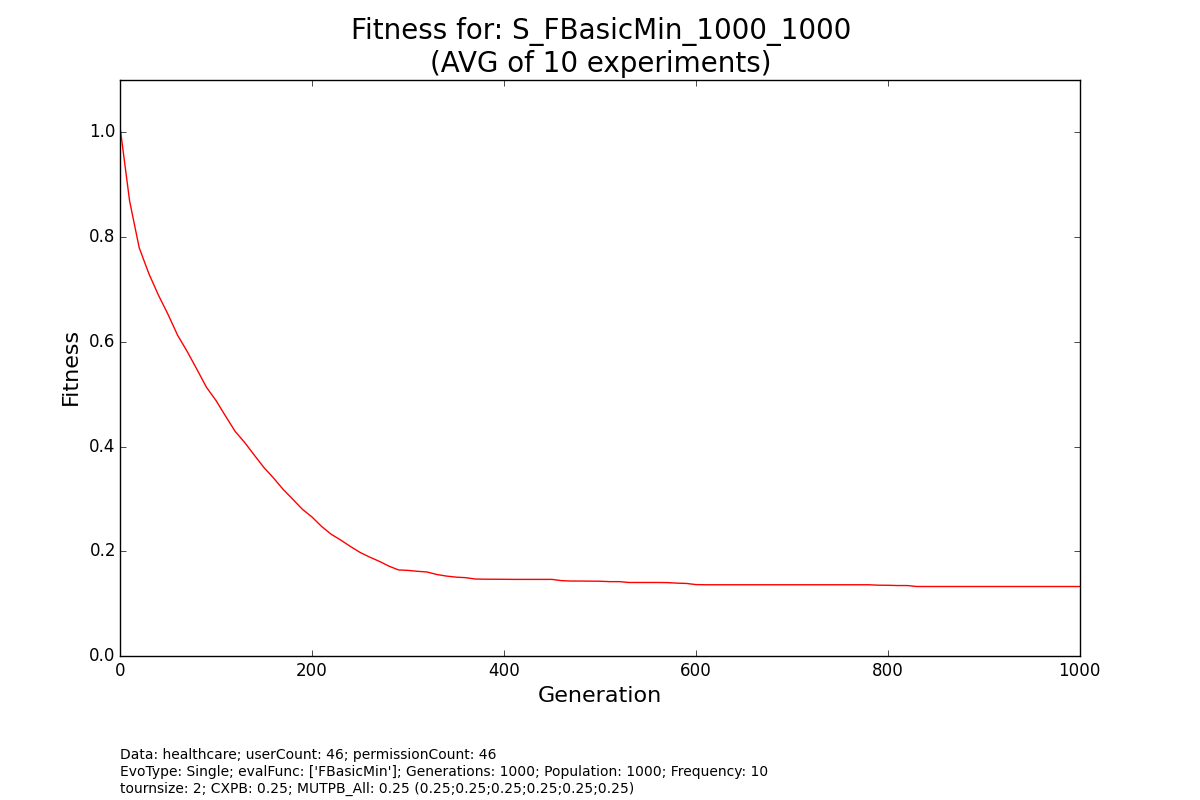
\includegraphics[scale=0.4, trim=0cm 2cm 0cm 0cm, clip=true]{exp2c_Fitness}
	    	\caption{EXPERIMENT 2c: Average minimum Fitness Graph of ten experiments with fitness function $F_{basic}^{min}$ and healthcare dataset}
	    	\label{fig:exp2c_Fitness}
		\end{figure}

\section{Experiment 2d}
\label{sec:A_Exp2d}
	\subsection{Result Data}
	\label{sec:A_Exp2d_Data}
		\begin{table}[H]
			\caption{Results of Experiment 2d: Healthcare Dataset, $F_{Edge}^{INT}$, Setup 1}
			\label{tab:A_Exp2d_Data}
			\begin{adjustbox}{max width=380pt,keepaspectratio,angle=90}
				\begin{tabular}{|l|l|l|l|l|l|l|l|l|l|l|}
					\rowcolor[HTML]{EFEFEF} 
					\hline
					Experiment & evals & Fitness\_Min & Fitness\_Max & Fitness\_Avg & Fitness\_Std & Conf\_Min & Conf\_Max & Conf\_Avg & Conf\_Std   & Accs\_Min \\ \hline
					1          & 440   & 0.122094308  & 0.652777475  & 0.148445876  & 0.073942818  & 5         & 313       & 14.563    & 36.09113508 & 56        \\ \hline
					2          & 441   & 0.123248421  & 0.610611923  & 0.149685959  & 0.06763063   & 16        & 266       & 23.673    & 28.61307518 & 67        \\ \hline
					3          & 459   & 0.127405752  & 0.613321023  & 0.148798701  & 0.061634077  & 0         & 282       & 12.531    & 29.8048157  & 58        \\ \hline
					4          & 452   & 0.093314057  & 0.637202857  & 0.116263647  & 0.065041304  & 5         & 297       & 13.28     & 32.23950372 & 40        \\ \hline
					5          & 449   & 0.120162874  & 0.525440678  & 0.140486656  & 0.057612971  & 5         & 271       & 13.19     & 31.11407881 & 46        \\ \hline
					6          & 444   & 0.110944496  & 0.627823762  & 0.126268738  & 0.050248204  & 10        & 319       & 18.644    & 28.01548258 & 35        \\ \hline
					7          & 455   & 0.140641126  & 0.657918404  & 0.162385924  & 0.067111664  & 4         & 327       & 16.918    & 31.17180258 & 37        \\ \hline
					8          & 433   & 0.135131489  & 0.602258371  & 0.151203818  & 0.052246174  & 0         & 305       & 10.006    & 23.94201253 & 60        \\ \hline
					9          & 433   & 0.12686091   & 0.497834593  & 0.14489562   & 0.053041654  & 0         & 239       & 8.977     & 29.78826062 & 64        \\ \hline
					10         & 453   & 0.124793266  & 0.536038771  & 0.141382439  & 0.051006272  & 0         & 247       & 6.705     & 27.88777465 & 62        \\ \hline\hline
					AVG        & 445.9 & 0.12245967   & 0.596122786  & 0.142981738  & 0.059951577  & 4.5       & 286.6     & 13.8487   & 29.86679414 & 52.5      \\ \hline
				\end{tabular}
			\end{adjustbox}
			\begin{adjustbox}{max width=380pt,keepaspectratio,angle=90}
				\begin{tabular}{|l|l|l|l|l|l|l|l|l|l|l|}
					\rowcolor[HTML]{EFEFEF} 
					\hline
					Experiment & Accs\_Max & Accs\_Avg & Accs\_Std   & RoleCnt\_Min & RoleCnt\_Max & RoleCnt\_Avg & RoleCnt\_Std & URCnt\_Min & URCnt\_Max & URCnt\_Avg \\ \hline
					1          & 542       & 130.46    & 64.14480805 & 3            & 6            & 4.016        & 0.334281319  & 63         & 127        & 93.667     \\ \hline
					2          & 473       & 122.756   & 76.4776599  & 3            & 6            & 4.018        & 0.357317786  & 63         & 117        & 80.422     \\ \hline
					3          & 417       & 127.939   & 49.77868298 & 4            & 6            & 4.991        & 0.344846343  & 69         & 126        & 94.775     \\ \hline
					4          & 361       & 101.391   & 53.52397705 & 2            & 6            & 3.019        & 0.344440125  & 47         & 107        & 66.252     \\ \hline
					5          & 337       & 124.957   & 39.13327422 & 3            & 5            & 3.992        & 0.343418113  & 48         & 103        & 71.756     \\ \hline
					6          & 270       & 74.845    & 27.51350532 & 4            & 6            & 5.007        & 0.314564779  & 69         & 124        & 91.205     \\ \hline
					7          & 628       & 129.756   & 67.40009246 & 4            & 6            & 5.004        & 0.322465502  & 75         & 145        & 114.852    \\ \hline
					8          & 520       & 126.496   & 54.14161047 & 4            & 6            & 4.99         & 0.303150128  & 55         & 111        & 79.069     \\ \hline
					9          & 294       & 121.788   & 28.74239127 & 3            & 6            & 5.003        & 0.324023147  & 67         & 144        & 113        \\ \hline
					10         & 402       & 122.901   & 33.35936449 & 3            & 6            & 4.989        & 0.32996818   & 67         & 143        & 110.832    \\ \hline\hline
					AVG        & 424.4     & 118.3289  & 49.42153662 & 3.3          & 5.9          & 4.5029       & 0.331847542  & 62.3       & 124.7      & 91.583     \\ \hline
				\end{tabular}	
			\end{adjustbox}
			\begin{adjustbox}{max width=380pt,keepaspectratio,angle=90}
				\begin{tabular}{|l|l|l|l|l|l|l|l|l|l|l|}
					\rowcolor[HTML]{EFEFEF} 
					\hline
					Experiment & URCnt\_Std  & RPCnt\_Min & RPCnt\_Max & RPCnt\_Avg & RPCnt\_Std  & Interp\_Min & Interp\_Max & Interp\_Avg & Interp\_Std & Runtime     \\ \hline
					1          & 7.462714721 & 50         & 118        & 69.596     & 6.207316973 & 0           & 0           & 0           & 0           & 750.174128  \\ \hline
					2          & 6.558804464 & 45         & 97         & 66.239     & 7.180381536 & 0           & 0           & 0           & 0           & 718.898073  \\ \hline
					3          & 6.503258798 & 63         & 113        & 79.399     & 5.554079492 & 0           & 0           & 0           & 0           & 820.277028  \\ \hline
					4          & 6.36007044  & 52         & 117        & 75.058     & 7.190732647 & 0           & 0           & 0           & 0           & 692.369822  \\ \hline
					5          & 6.842694206 & 70         & 120        & 87.194     & 5.871657688 & 0           & 0           & 0           & 0           & 732.606132  \\ \hline
					6          & 6.038292391 & 72         & 120        & 90.192     & 5.105402629 & 0           & 0           & 0           & 0           & 796.778843  \\ \hline
					7          & 6.599552712 & 37         & 104        & 70.532     & 5.899235205 & 0           & 0           & 0           & 0           & 826.102517  \\ \hline
					8          & 5.32524544  & 77         & 144        & 110.383    & 6.907409862 & 0           & 0           & 0           & 0           & 796.886848  \\ \hline
					9          & 6.6938778   & 51         & 105        & 73.322     & 5.59234441  & 0           & 0           & 0           & 0           & 819.119086  \\ \hline
					10         & 6.078632741 & 49         & 106        & 74.121     & 6.022819855 & 0           & 0           & 0           & 0           & 798.321932  \\ \hline\hline
					AVG        & 6.446314371 & 56.6       & 114.4      & 79.6036    & 6.153138029 & 0           & 0           & 0           & 0           & 775.1534409 \\ \hline
				\end{tabular}
			\end{adjustbox}	
		\end{table}
	\subsection{Result Visualizations}
	\label{sec:A_Exp2d_Diagrams}
		\begin{figure}[H]
			\centering
			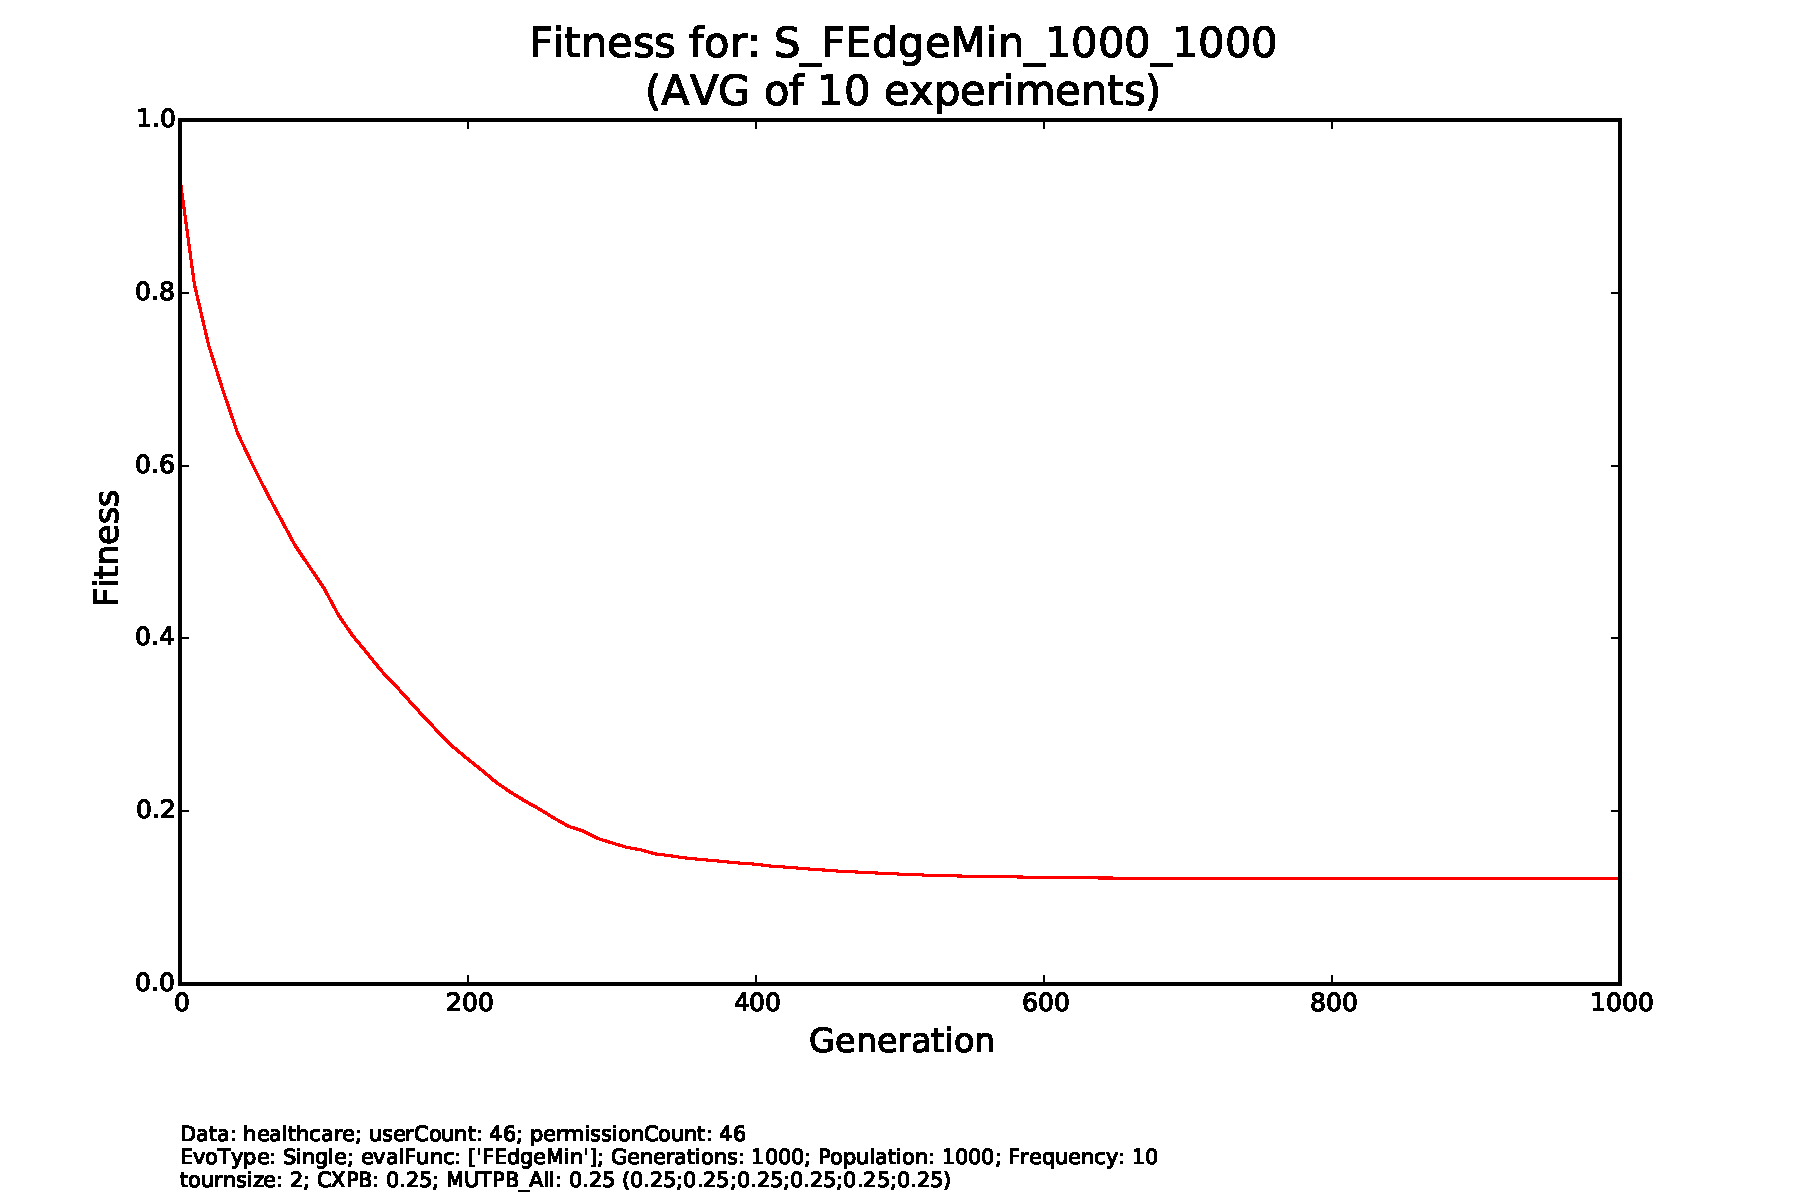
\includegraphics[scale=0.4, trim=0cm 2cm 0cm 0cm, clip=true]{exp2d_Fitness}
			\caption{EXPERIMENT 2d: Average minimum Fitness Graph of ten experiments with fitness function $F_{edge}^{min}$ and healthcare dataset}
			\label{fig:exp2d_Fitness}
		\end{figure}

\section{Experiment 3a}
\label{sec:A_Exp3a}
	\subsection{Result Data}
	\label{sec:A_Exp3a_Data}
	\subsection{Result Visualizations}
	\label{sec:A_Exp3a_Diagrams}
		\begin{figure}[H]
			\centering
			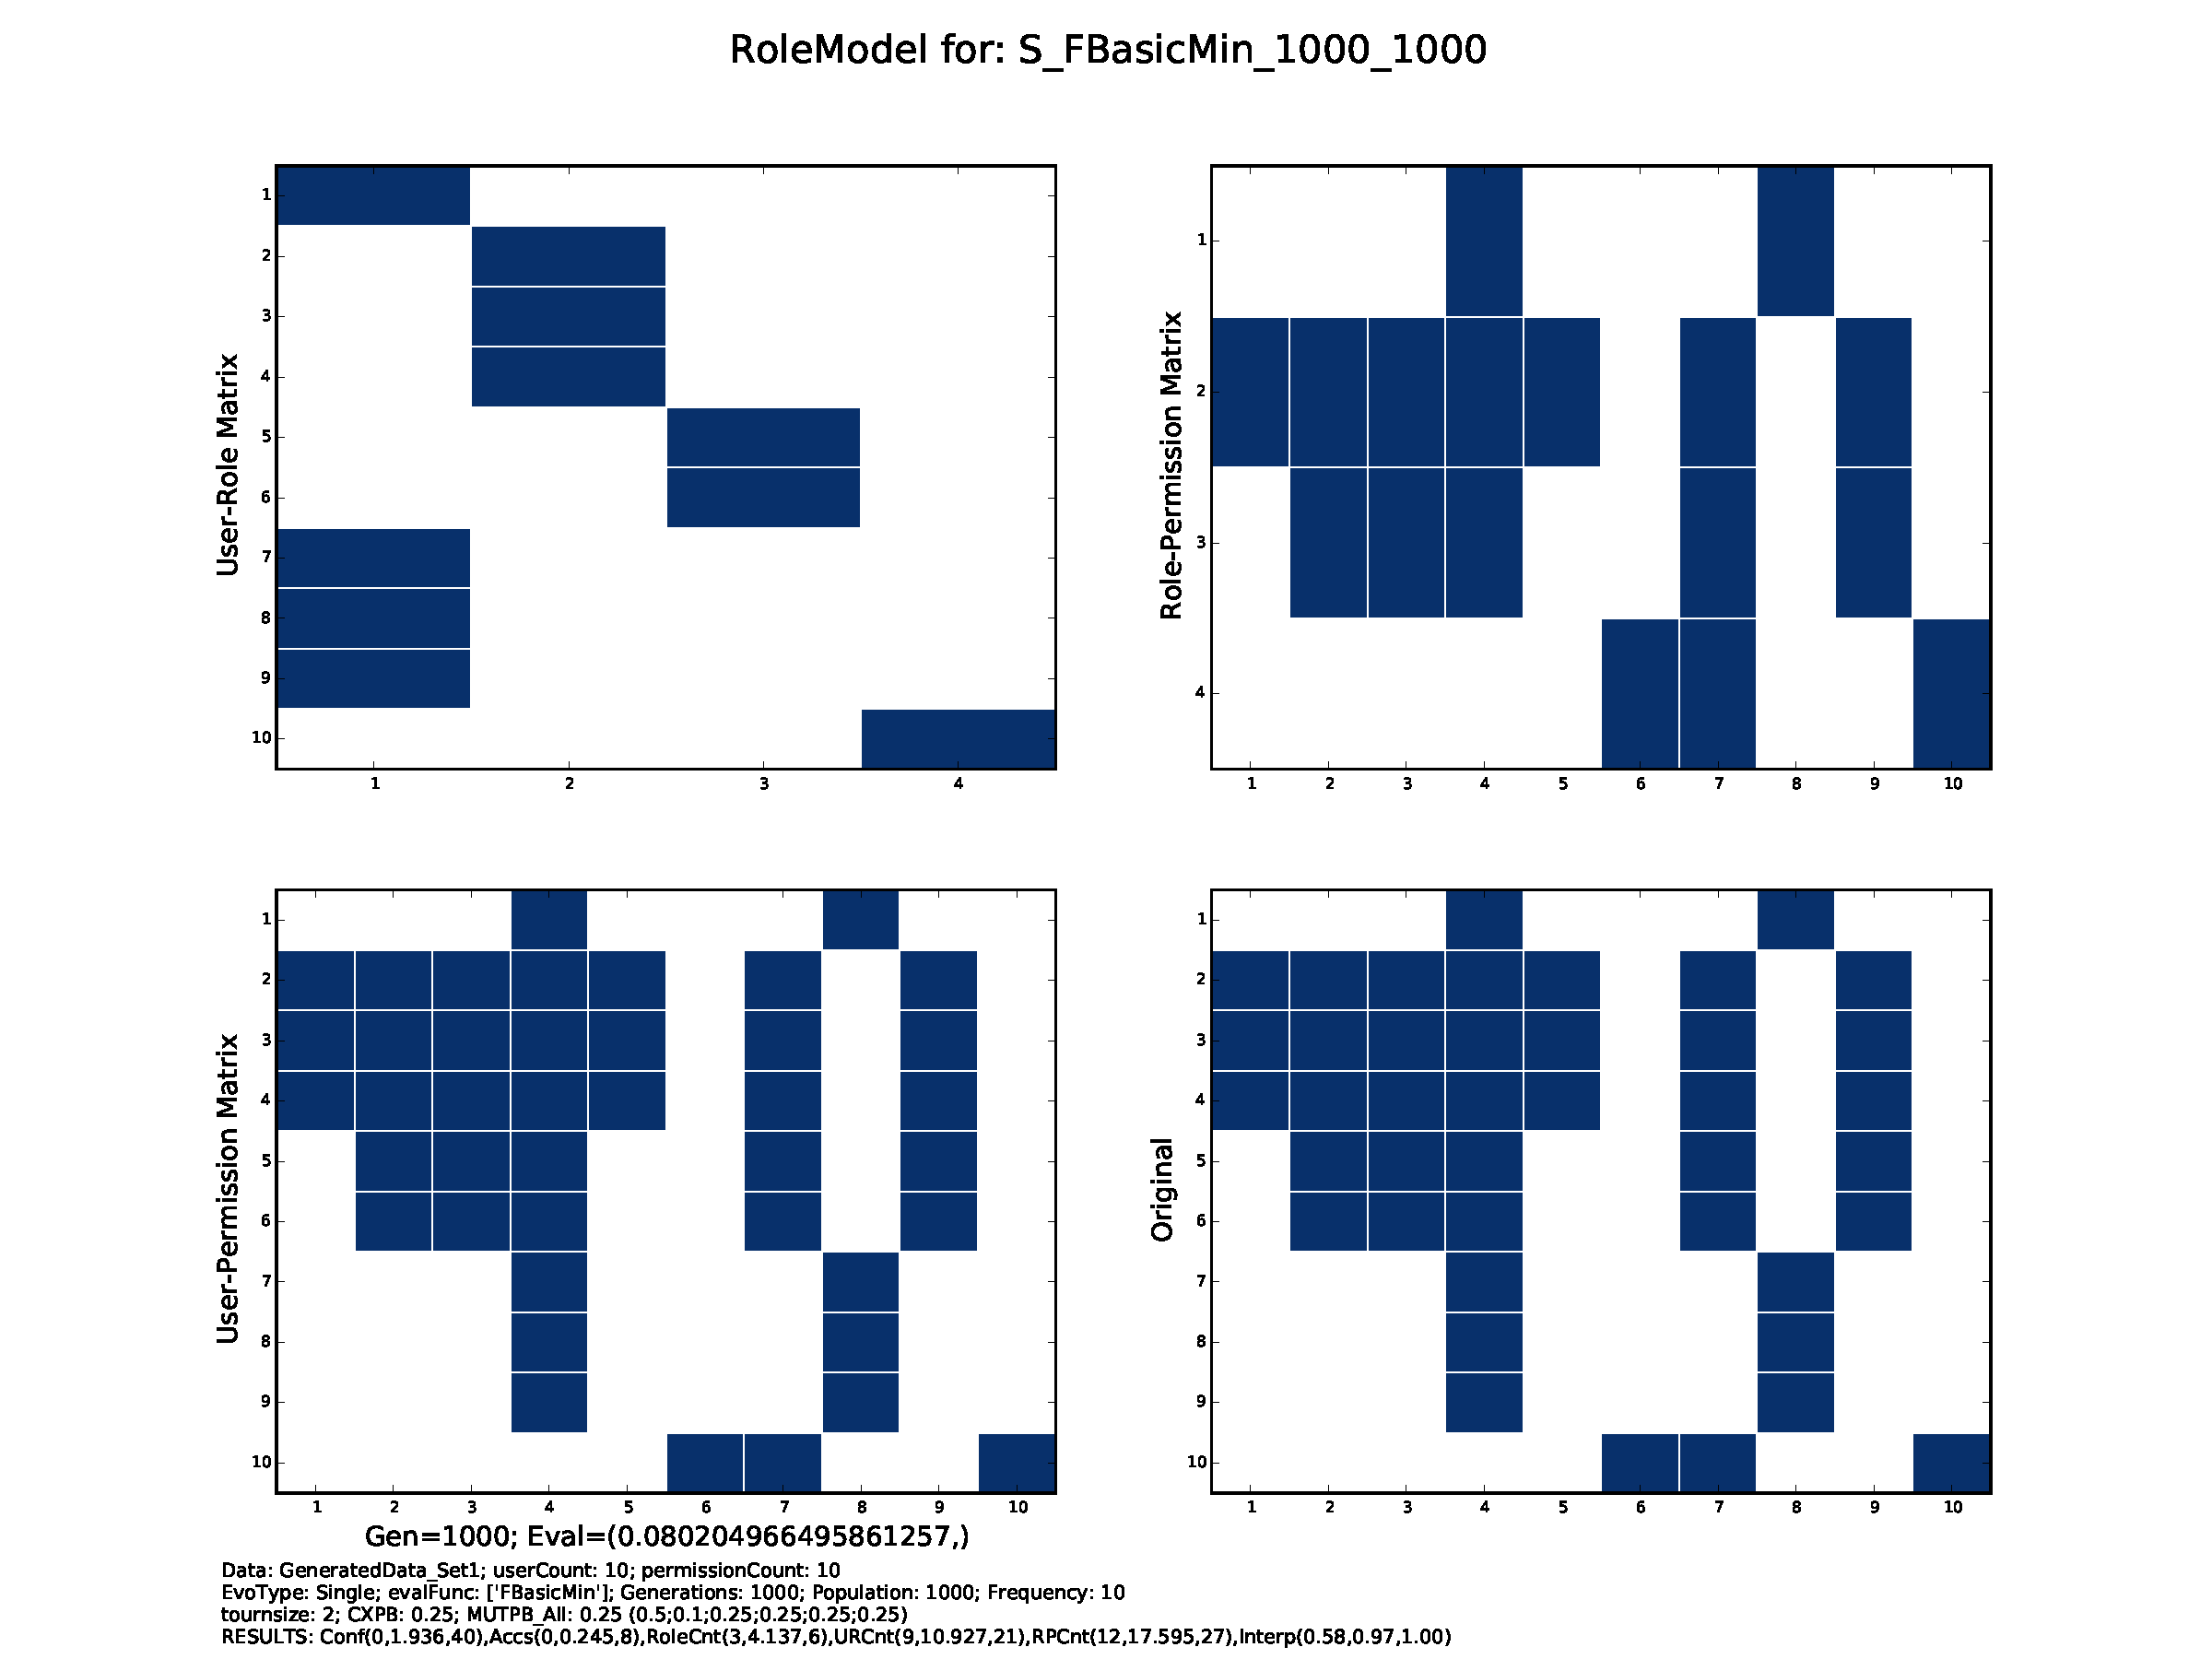
\includegraphics[scale=0.37, trim=4cm 2cm 4cm 2cm, clip=true]{exp3a_RM}
			\caption{EXPERIMENT 3a: Example of fitness-optimal solution role model resulting of EvoRoleMiner with Fitness function $F_{basic}^{min}$ on synthetic dataset 1 with setup in table \ref{tab:exp3_setup}. From u.l. to l.r.: User-Role Matrix, Role-Permission Matrix, Resulting User-Permission Matrix, Original User-Permission Matrix from Input. A blue box stands for an assignment. The darker the blue the more usre-role- and role-permission assignments causing the user-permission assignment.}
			\label{fig:exp3a_RM}
		\end{figure}

\section{Experiment 3b}
\label{sec:A_Exp3b}
	\subsection{Result Data}
	\label{sec:A_Exp3b_Data}
	\subsection{Result Visualizations}
	\label{sec:A_Exp3b_Diagrams}
		\begin{figure}[H]
			\centering
			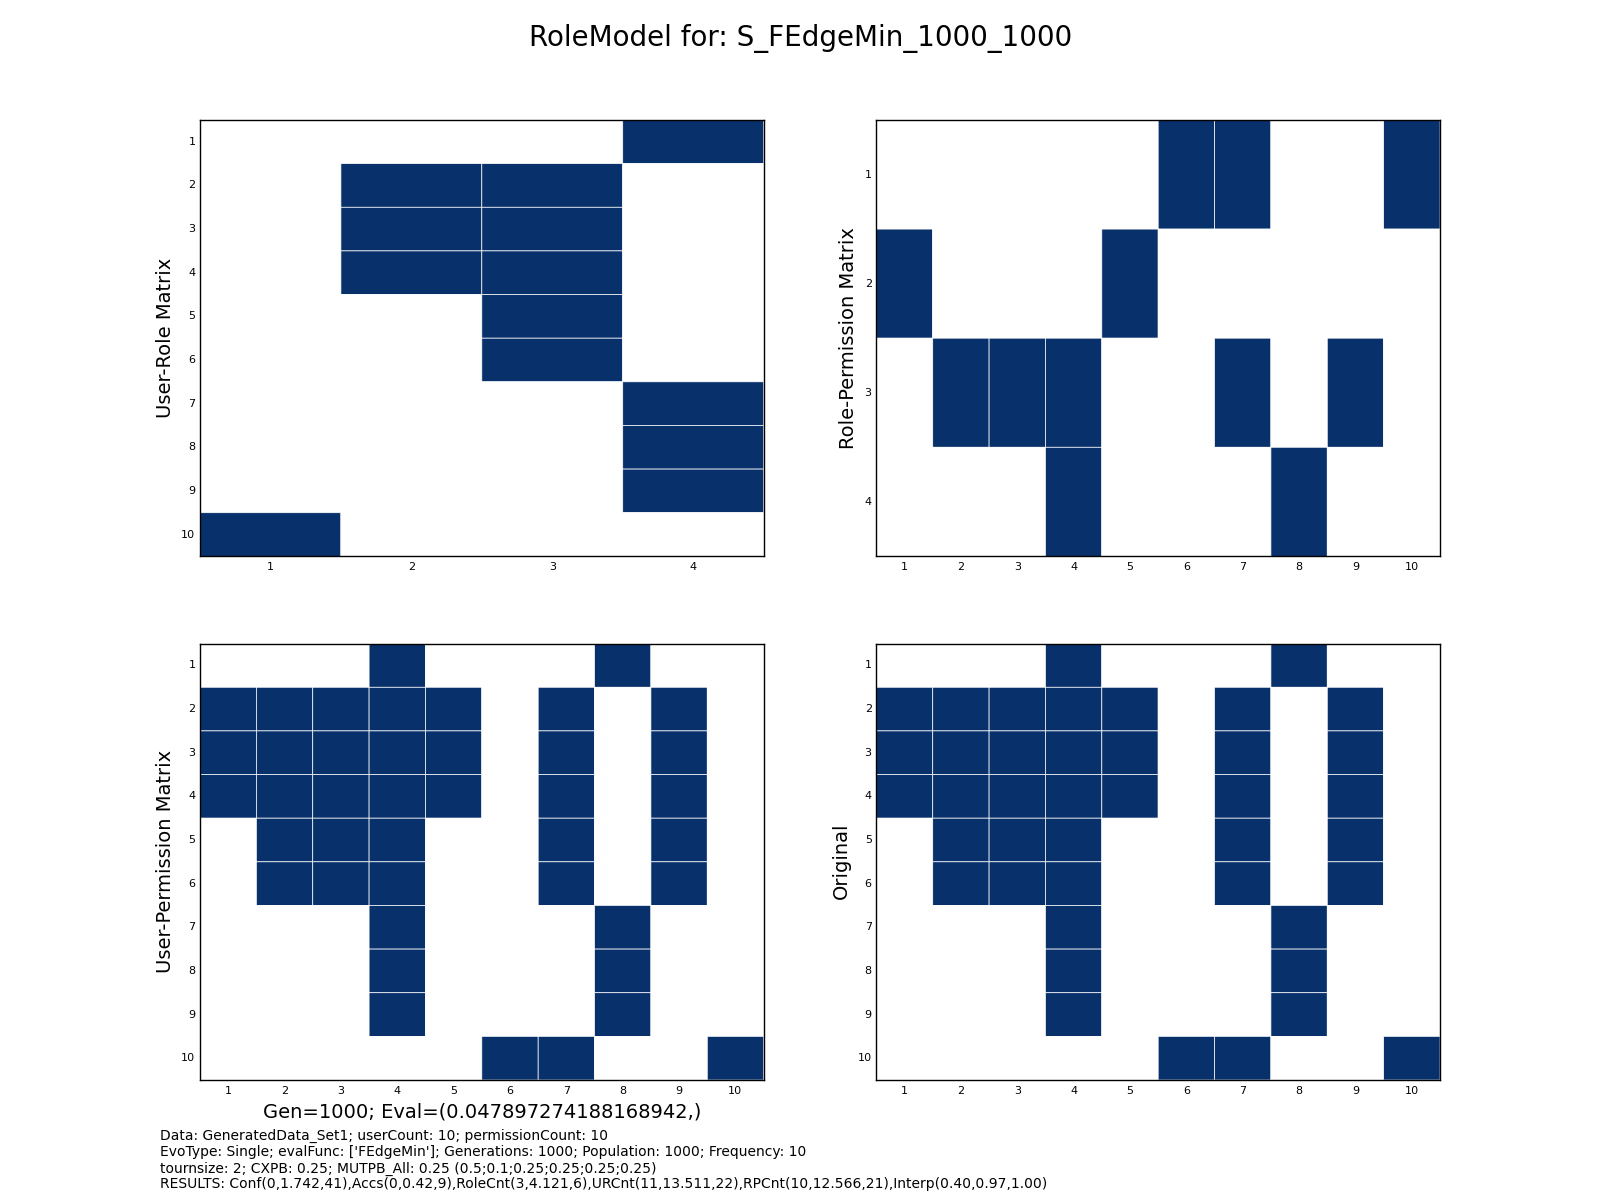
\includegraphics[scale=0.37, trim=4cm 2cm 4cm 2cm, clip=true]{exp3b_RM}
			\caption{EXPERIMENT 3b: Example of fitness-optimal solution role model resulting of EvoRoleMiner with Fitness function $F_{edge}^{min}$ on synthetic dataset 1 with setup in table \ref{tab:exp3_setup}. From u.l. to l.r.: User-Role Matrix, Role-Permission Matrix, Resulting User-Permission Matrix, Original User-Permission Matrix from Input. A blue box stands for an assignment. The darker the blue the more usre-role- and role-permission assignments causing the user-permission assignment.}
			\label{fig:exp3b_RM}
		\end{figure}

\section{Experiment 3c}
\label{sec:A_Exp3c}
	\subsection{Result Data}
	\label{sec:A_Exp3c_Data}
	\subsection{Result Visualizations}
	\label{sec:A_Exp3c_Diagrams}

\section{Experiment 3d}
\label{sec:A_Exp3d}
	\subsection{Result Data}
	\label{sec:A_Exp3d_Data}
	\subsection{Result Visualizations}
	\label{sec:A_Exp3d_Diagrams}

\section{Experiment 4a}
\label{sec:A_Exp4a}
	\subsection{Result Data}
	\label{sec:A_Exp4a_Data}
	\subsection{Result Visualizations}
	\label{sec:A_Exp4a_Diagrams}
		\begin{figure}[H]
			\centering
			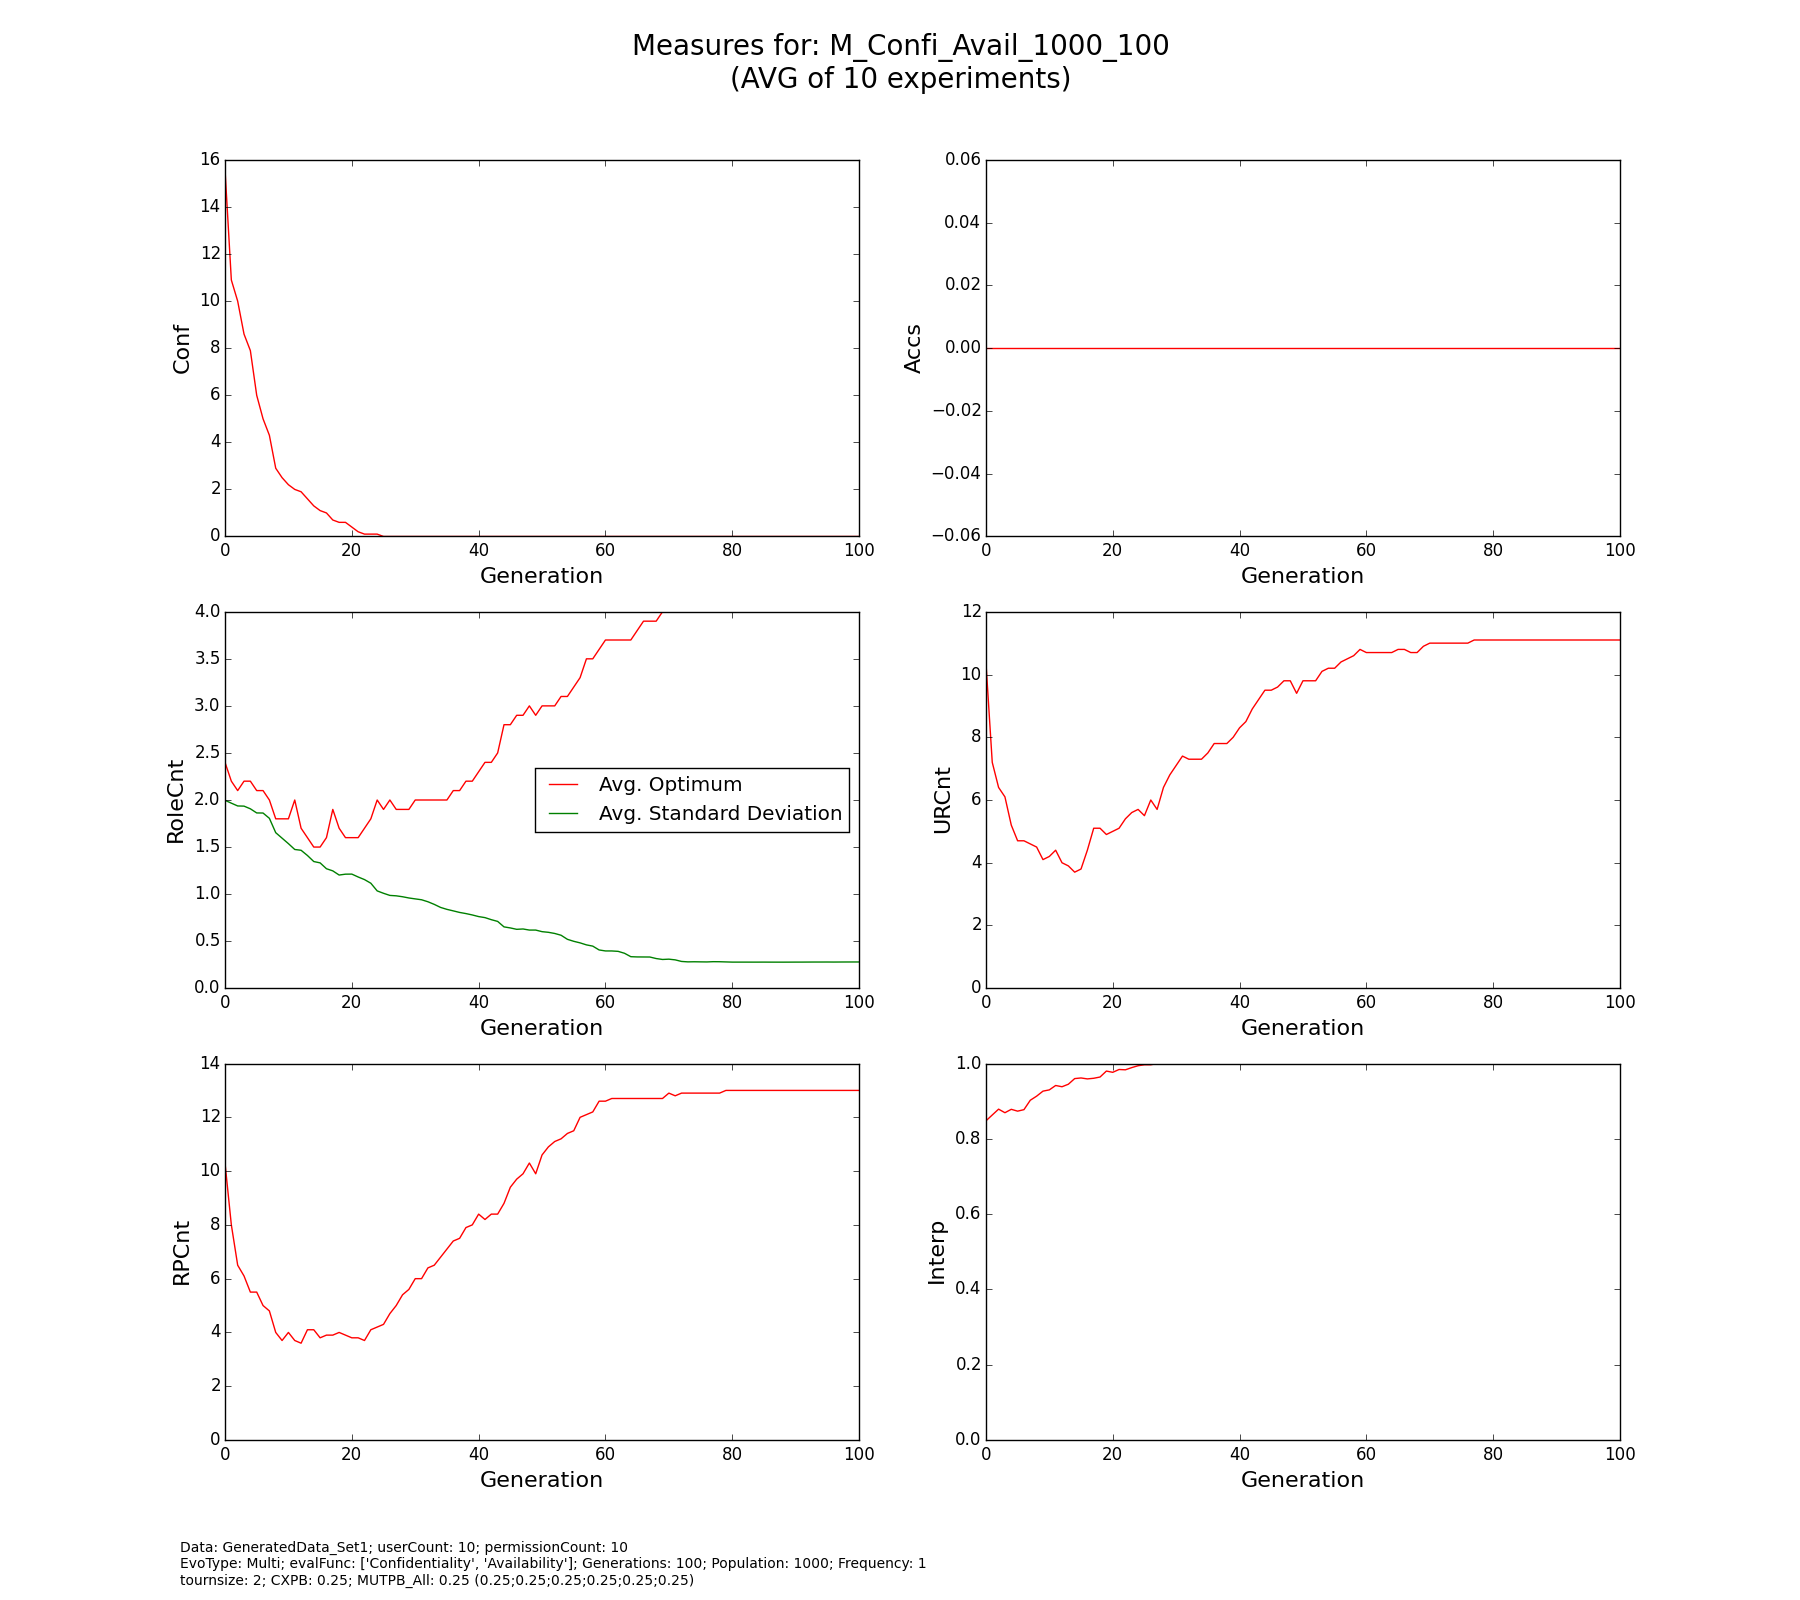
\includegraphics[scale=0.33, trim=4cm 2cm 4cm 0cm, clip=true]{exp4a_measures}
			\caption{EXPERIMENT 4a: Average optimum of the single objective measures of the ten experiments with Evo-RoleMiner$M$ on Dataset1}
			\label{fig:exp4a_measures}
		\end{figure}
		\begin{figure}[H]
			\centering
			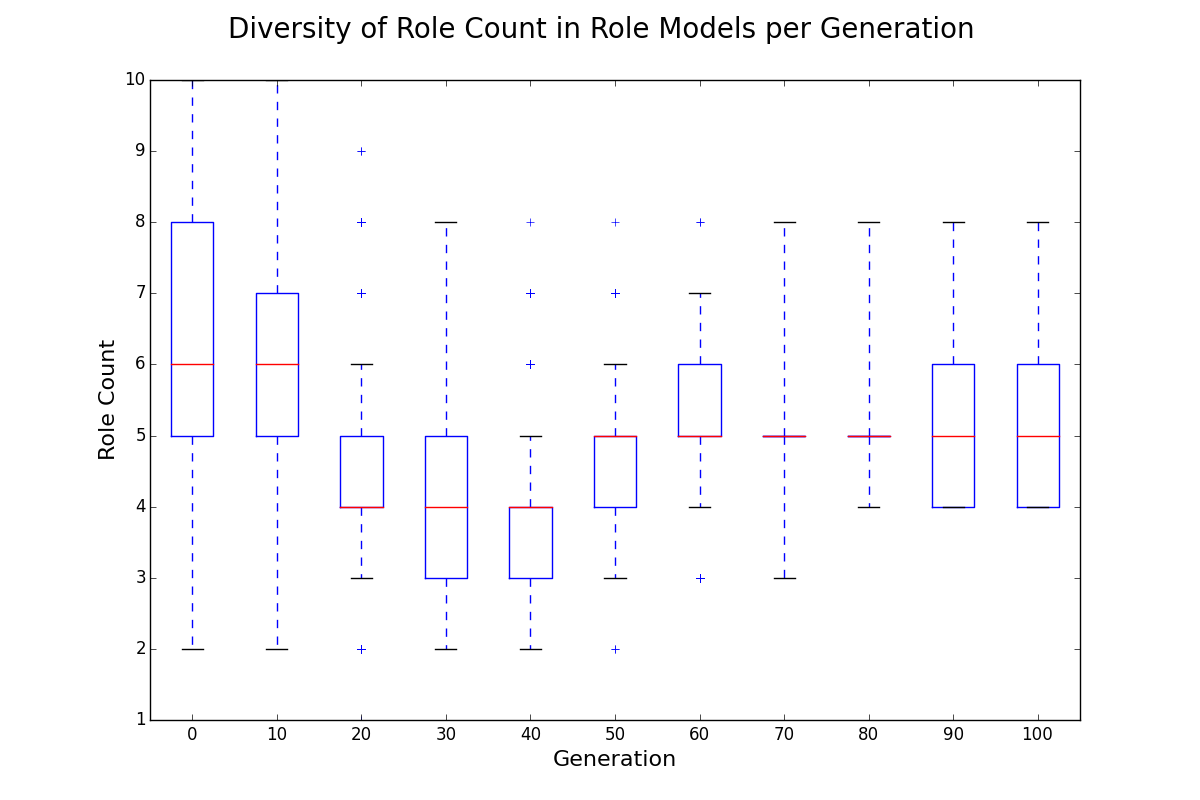
\includegraphics[scale=0.3]{exp4a_diversity}
			\caption{EXPERIMENT 4a: Example boxplot of role count diversity of individuals of a population in different generations with Evo-RoleMiner$M$ on Dataset1.}
			\label{fig:exp4a_diversity}
		\end{figure}

\section{Experiment 4b}
\label{sec:A_Exp4b}
	\subsection{Result Data}
	\label{sec:A_Exp4b_Data}
	\subsection{Result Visualizations}
	\label{sec:A_Exp4b_Diagrams}

\section{Experiment 4c}
\label{sec:A_Exp4c}
	\subsection{Result Data}
	\label{sec:A_Exp4c_Data}
	\subsection{Result Visualizations}
	\label{sec:A_Exp4c_Diagrams}
		\begin{figure}[H]
			\centering
			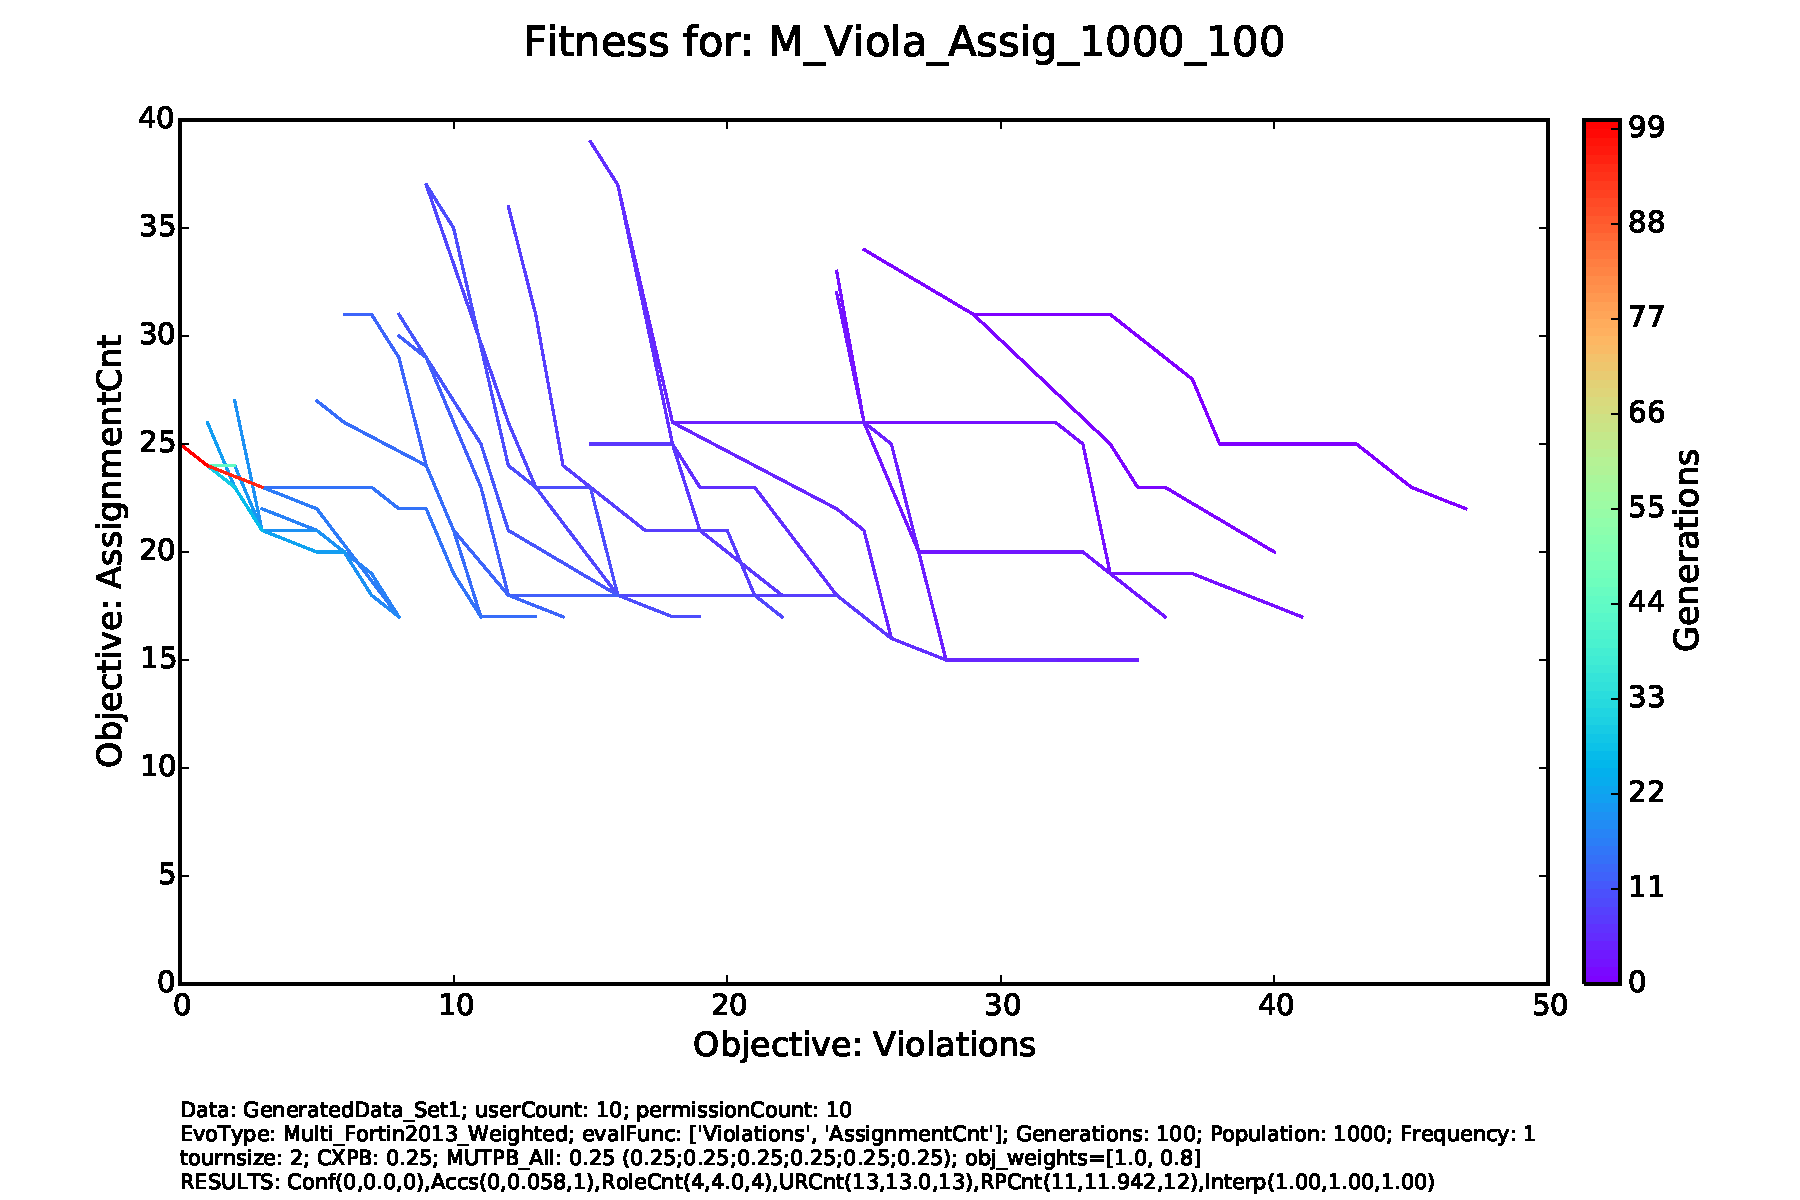
\includegraphics[width=\textwidth, trim=0cm 2cm 0cm 1.5cm, clip=true]{exp4c_fitness_pareto}
			\caption{EXPERIMENT 4c: Example of result of the experiments with Evo-RoleMiner$M$ on the Healthcare dataset. Illustrates the pareto fronts of each generation.}
			\label{fig:exp4c_fitness_pareto}
		\end{figure}
		\begin{figure}[H]
			\centering
			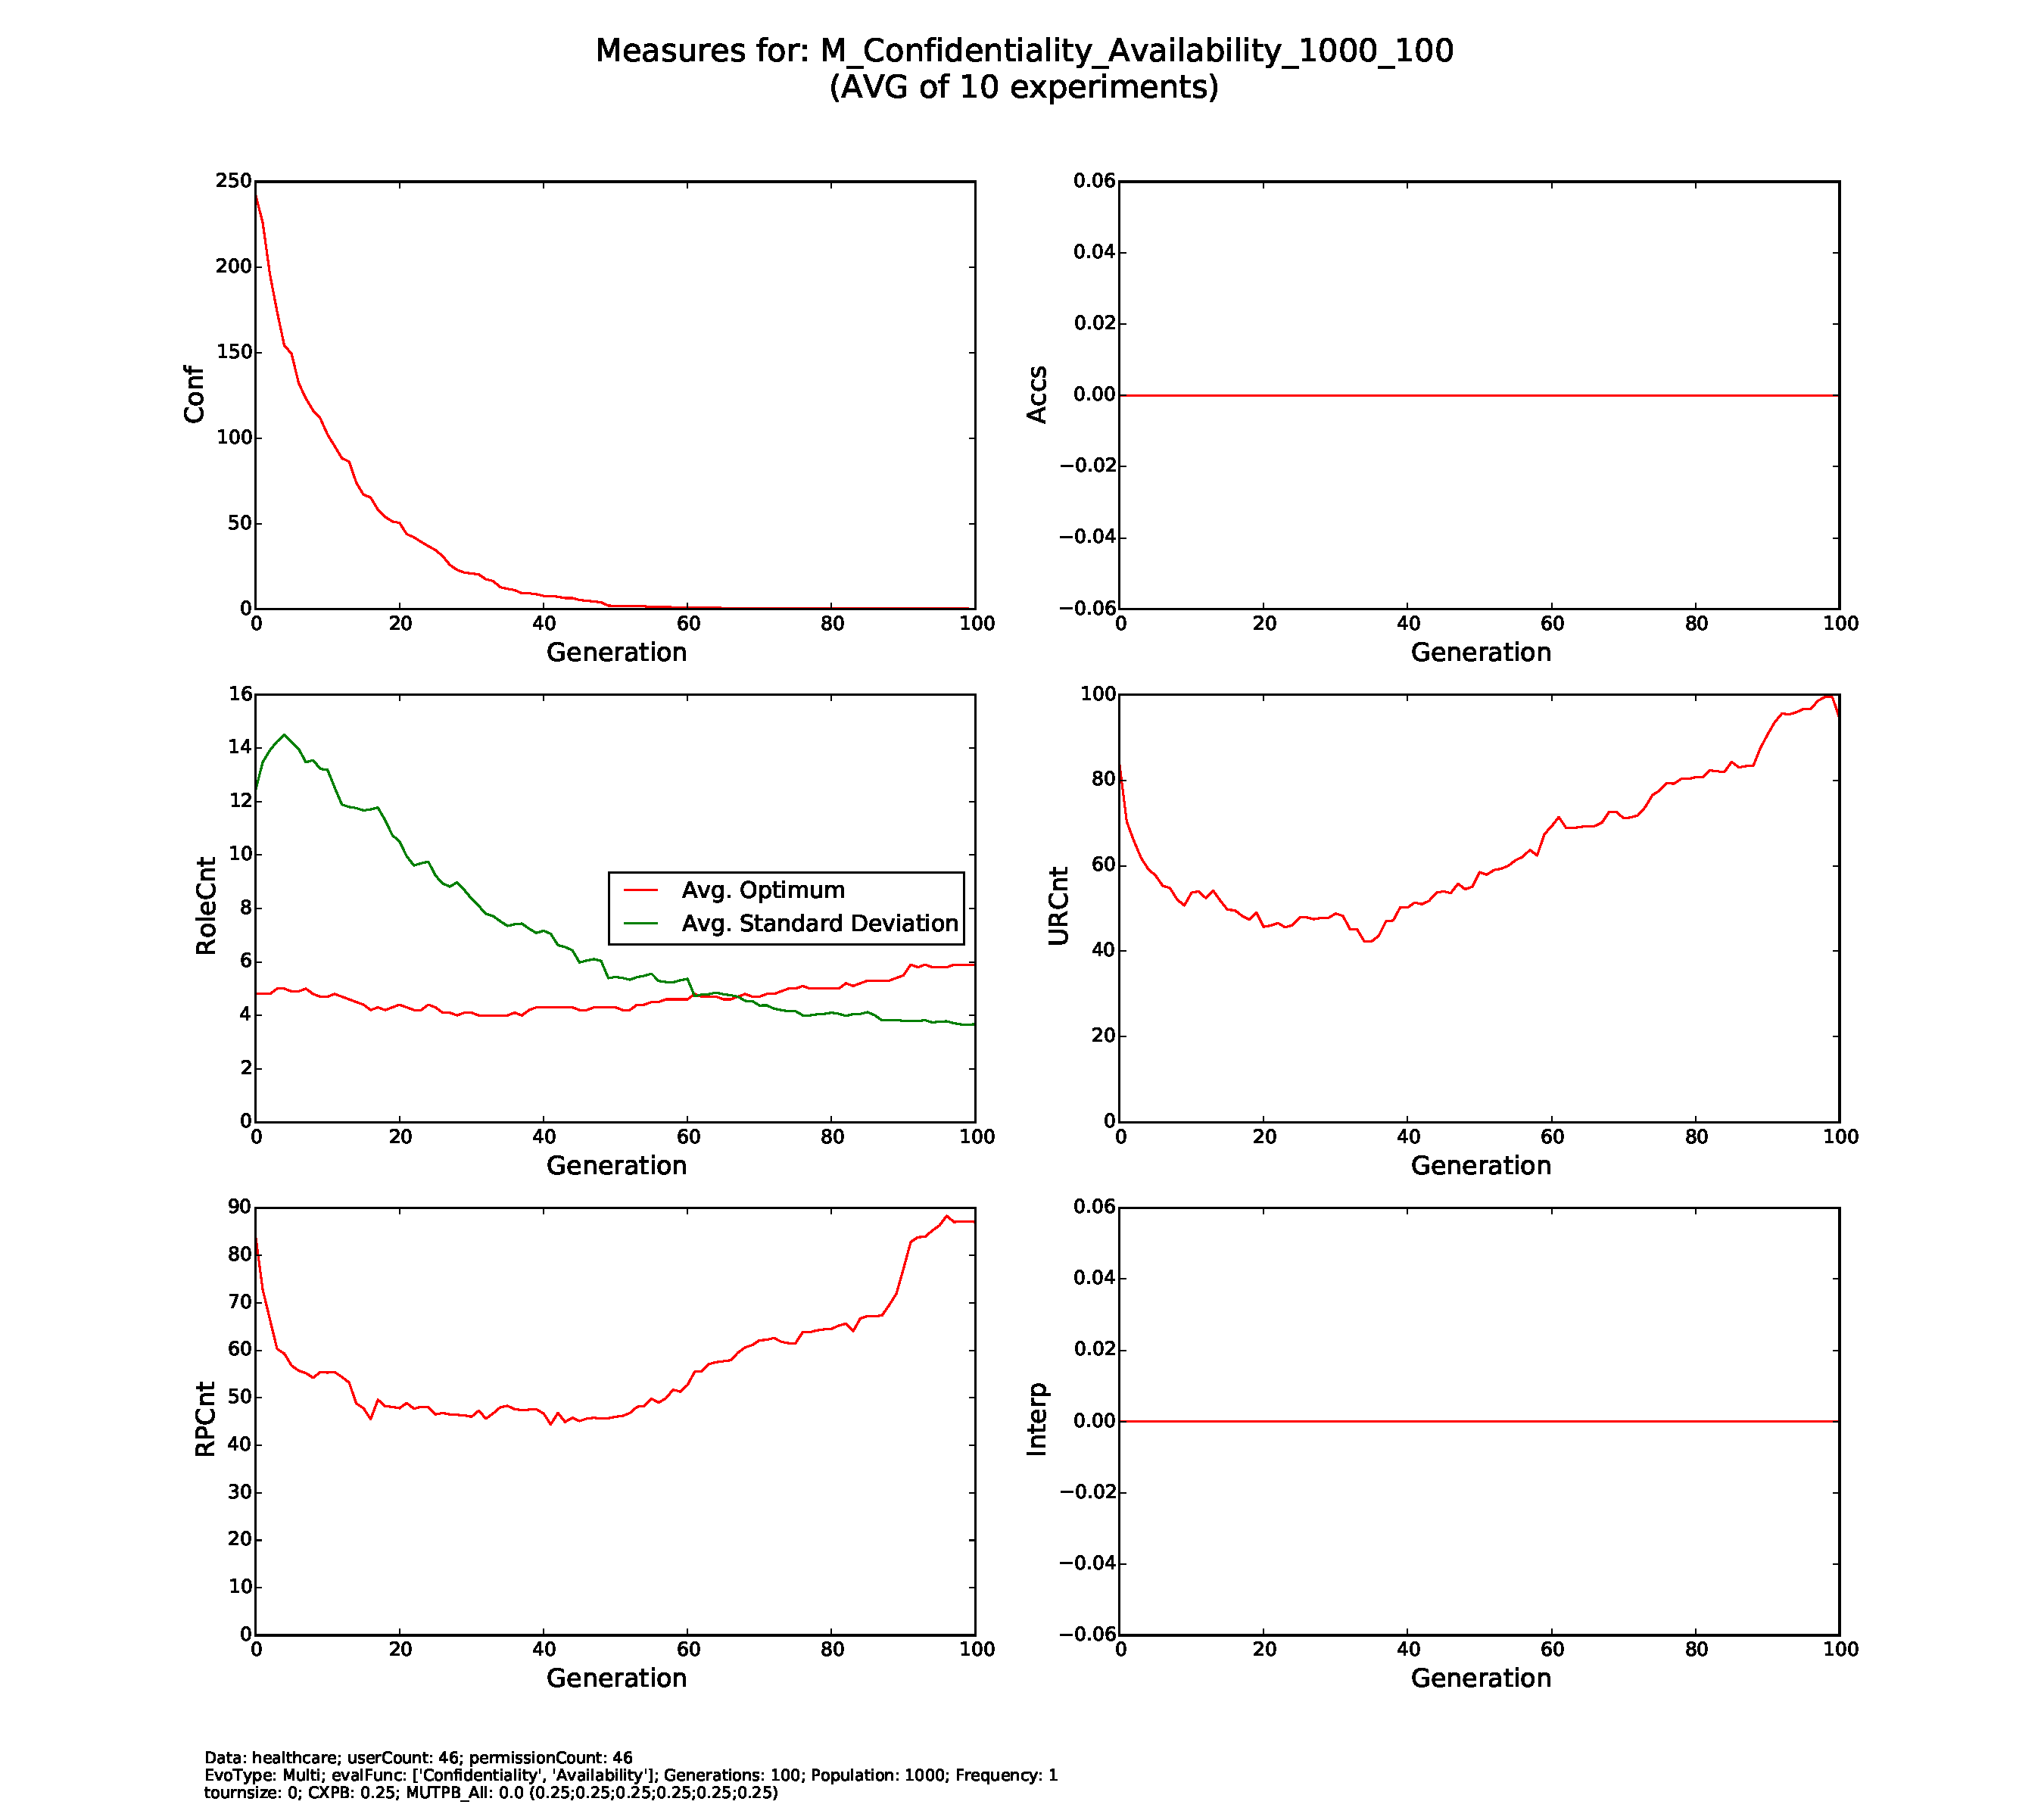
\includegraphics[scale=0.33, trim=4cm 2cm 4cm 0cm, clip=true]{exp4c_measures}
			\caption{EXPERIMENT 4c: Average optimum of the single objective measures of the ten experiments with Evo-RoleMiner$M$ on the healthcare dataset. The Interpretability measure is not activated and therefore constantly zero.}
			\label{fig:exp4c_measures}
		\end{figure}

\section{Experiment 4d}
\label{sec:A_Exp4d}
	\subsection{Result Data}
	\label{sec:A_Exp4d_Data}
	\subsection{Result Visualizations}
	\label{sec:A_Exp4d_Diagrams}